\documentclass{beamer}
\usepackage[utf8]{inputenc}
\usepackage{graphicx, epsfig}
\usepackage{amsmath,mathrsfs,amsfonts,amssymb}
\usepackage{floatflt}
\usepackage{epic,ecltree}
\usepackage{mathtext}
\usepackage{fancybox}
\usepackage{fancyhdr}
\usepackage{multirow}
\usepackage{enumerate}
\usepackage{epstopdf}
\usepackage{multicol}
\usepackage{algorithm}
\usepackage[noend]{algorithmic}
\usepackage{tikz}
\usepackage{blindtext}
\usetheme{default}%{Singapore}%{Warsaw}%{Warsaw}%{Darmstadt}
\usecolortheme{default}

\setbeamerfont{title}{size=\Huge}
\setbeamertemplate{footline}[page number]{}

\setbeamertemplate{section in toc}[sections numbered]


\makeatletter
\newcommand\HUGE{\@setfontsize\Huge{35}{40}}
\makeatother    

\setbeamerfont{title}{size=\HUGE}
\beamertemplatenavigationsymbolsempty

% latin bold lower
\newcommand{\ba}{\mathbf{a}} 
\newcommand{\bc}{\mathbf{c}} 
\newcommand{\be}{\mathbf{e}} 
\newcommand{\bh}{\mathbf{h}} 
\newcommand{\bp}{\mathbf{p}} 
\newcommand{\bt}{\mathbf{t}} 
\newcommand{\bs}{\mathbf{s}} 
\newcommand{\bu}{\mathbf{u}} 
\newcommand{\bv}{\mathbf{v}} 
\newcommand{\bw}{\mathbf{w}} 
\newcommand{\bx}{\mathbf{x}} 
\newcommand{\by}{\mathbf{y}} 
\newcommand{\bz}{\mathbf{z}} 

% latin bold upper
\newcommand{\bA}{\mathbf{A}} 
\newcommand{\bB}{\mathbf{B}} 
\newcommand{\bC}{\mathbf{C}} 
\newcommand{\bI}{\mathbf{I}} 
\newcommand{\bJ}{\mathbf{J}} 
\newcommand{\bL}{\mathbf{L}} 
\newcommand{\bM}{\mathbf{M}} 
\newcommand{\bP}{\mathbf{P}}
\newcommand{\bQ}{\mathbf{Q}} 
\newcommand{\bR}{\mathbf{R}} 
\newcommand{\bT}{\mathbf{T}} 
\newcommand{\bU}{\mathbf{U}} 
\newcommand{\bV}{\mathbf{V}} 
\newcommand{\bW}{\mathbf{W}} 
\newcommand{\bX}{\mathbf{X}} 
\newcommand{\bY}{\mathbf{Y}} 
\newcommand{\bZ}{\mathbf{Z}} 

% latin cal upper
\newcommand{\cF}{\mathcal{F}} 
\newcommand{\cG}{\mathcal{G}} 
\newcommand{\cI}{\mathcal{I}} 
\newcommand{\cL}{\mathcal{L}} 
\newcommand{\cM}{\mathcal{M}} 
\newcommand{\cN}{\mathcal{N}} 
\newcommand{\cS}{\mathcal{S}} 
\newcommand{\cT}{\mathcal{T}} 
\newcommand{\cW}{\mathcal{W}} 
\newcommand{\cX}{\mathcal{X}} 
\newcommand{\cZ}{\mathcal{Z}} 

% latin bb upper
\newcommand{\bbE}{\mathbb{E}} 
\newcommand{\bbI}{\mathbb{I}} 
\newcommand{\bbP}{\mathbb{P}} 
\newcommand{\bbR}{\mathbb{R}} 

% greek bold lower
\newcommand{\bepsilon}{\boldsymbol{\epsilon}} 
\newcommand{\btheta}{\boldsymbol{\theta}} 
\newcommand{\blambda}{\boldsymbol{\lambda}} 
\newcommand{\bpi}{\boldsymbol{\pi}} 
\newcommand{\bmu}{\boldsymbol{\mu}} 
\newcommand{\bsigma}{\boldsymbol{\sigma}} 
\newcommand{\bphi}{\boldsymbol{\phi}} 

% greek bold upper
\newcommand{\bSigma}{\boldsymbol{\Sigma}} 

\DeclareMathOperator*{\argmin}{arg\,min}
\DeclareMathOperator*{\argmax}{arg\,max}

\newcommand{\createdgmtitle}[1]{\title[\hbox to 56mm{Deep Generative Models  \hfill\insertframenumber\,/\,\inserttotalframenumber}]
	{\vspace{1cm} \\ Deep Generative Models \\ {\Huge Lecture #1}}
	\author{Roman Isachenko}
	\institute{
	Moscow Institute of Physics and Technology
	} 
	\date{2023, Autumn}
}

\usepackage{tikz}
\usetikzlibrary{arrows,shapes,positioning,shadows,trees}

\newcommand\myfootnote[1]{%
  \tikz[remember picture,overlay]
  \draw (current page.south west) +(1in + \oddsidemargin,0.5em)
  node[anchor=south west,inner sep=0pt]{\parbox{\textwidth}{%
      \rlap{\rule{10em}{0.4pt}}\raggedright\scriptsize \textit{#1}}};}

\newcommand\myfootnotewithlink[2]{%
  \tikz[remember picture,overlay]
  \draw (current page.south west) +(1in + \oddsidemargin,0.5em)
  node[anchor=south west,inner sep=0pt]{\parbox{\textwidth}{%
      \rlap{\rule{10em}{0.4pt}}\raggedright\scriptsize\href{#1}{\textit{#2}}}};}
      
\AtBeginSection[]
      {
      	\begin{frame}{Outline}
      		\tableofcontents[currentsection]
      	\end{frame}
      }
      \AtBeginSubsection[]{
      	\begin{frame}{Outline}
      		\tableofcontents[currentsection,currentsubsection]
      	\end{frame}
}
\createdgmtitle{12}

\usepackage{tikz}

\usetikzlibrary{arrows,shapes,positioning,shadows,trees}
%--------------------------------------------------------------------------------
\begin{document}
%--------------------------------------------------------------------------------
\begin{frame}[noframenumbering,plain]
%\thispagestyle{empty}
\titlepage
\end{frame}
%=======
\begin{frame}{Recap of previous lecture}
	\begin{figure}
		\centering
		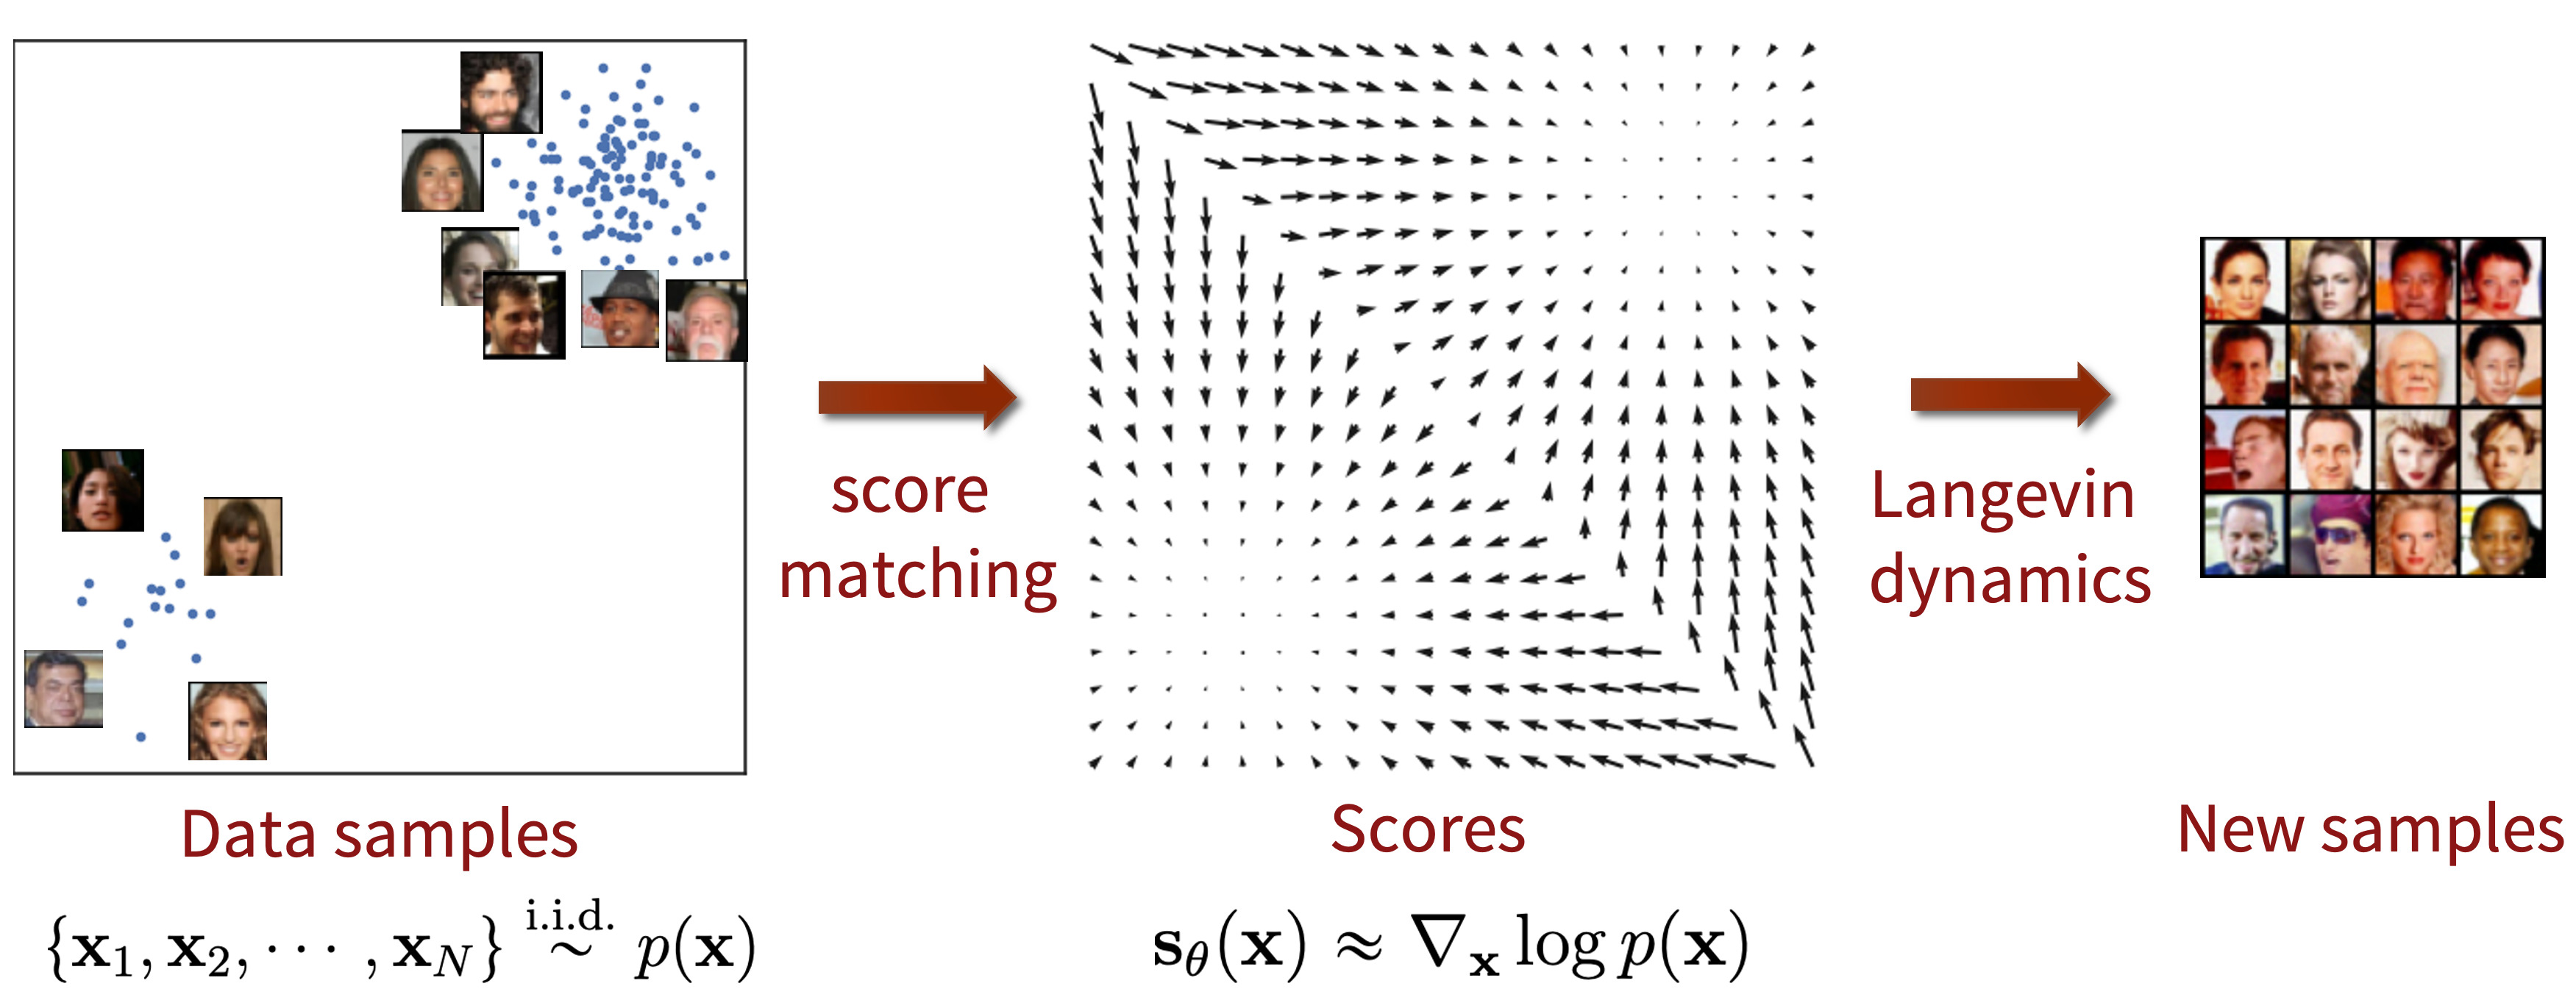
\includegraphics[width=0.75\linewidth]{figs/smld}
	\end{figure}
	\vspace{-0.3cm} 
	\begin{block}{Theorem (implicit score matching)}
		\vspace{-0.6cm}
		\[
		{\color{violet}\frac{1}{2} \bbE_{\pi}\bigl\| \bs_{\btheta}(\bx) - \nabla_\bx \log \pi(\bx) \bigr\|^2_2} = {\color{teal}\bbE_{\pi}\Bigr[ \frac{1}{2}\| \bs_{\btheta}(\bx) \|_2^2 + \text{tr}\bigl(\nabla_{\bx} \bs_{\btheta}(\bx)\bigr) \Bigr]} + \text{const}
		\]
	\end{block}
	\vspace{-0.5cm}
	\begin{enumerate}
		\item {\color{violet}The left hand side} is intractable due to unknown $\pi(\bx)$ -- \textbf{denoising score matching}. 
		\item {\color{teal}The right hand side} is complex due to Hessian matrix -- \textbf{sliced score matching (Hutchinson's trace estimation)}.
	\end{enumerate}
	\myfootnotewithlink{https://yang-song.github.io/blog/2021/score/}{Song Y. Generative Modeling by Estimating Gradients of the Data Distribution, blog post, 2021}
\end{frame}
%=======
\begin{frame}{Recap of previous lecture}
	Let perturb original data by normal noise $p(\bx' | \bx, \sigma) = \cN(\bx' | \bx, \sigma^2 \bI)$
	\vspace{-0.3cm}
	\[
	\pi(\bx' | \sigma) = \int \pi(\bx) p(\bx' | \bx, \sigma) d\bx.
	\]
	\vspace{-0.6cm} \\
	Then the solution of 
	\vspace{-0.2cm}
	\[
	\frac{1}{2} \bbE_{\pi(\bx' | \sigma)}\bigl\| \bs_{\btheta}(\bx', \sigma) - \nabla_{\bx'} \log \pi(\bx' | \sigma) \bigr\|^2_2 \rightarrow \min_{\btheta}
	\]
	\vspace{-0.5cm} \\
	satisfies $\bs_{\btheta}(\bx', \sigma) \approx \bs(\bx', \btheta, 0) = \bs(\bx', \btheta)$ if $\sigma$ is small enough.
	\begin{block}{Theorem (denoising score matching)}
		\vspace{-0.8cm}
		\begin{multline*}
			\bbE_{\pi(\bx' | \sigma)}\bigl\| \bs_{\btheta}(\bx', \sigma) - \nabla_{\bx'} \log \pi(\bx' | \sigma) \bigr\|^2_2 = \\ = \bbE_{\pi(\bx)} \bbE_{p(\bx' | \bx, \sigma)}\bigl\| \bs_{\btheta}(\bx', \sigma) - \nabla_{\bx'} \log p(\bx' | \bx, \sigma) \bigr\|^2_2 + \text{const}(\btheta)
		\end{multline*}
		\vspace{-0.8cm}
	\end{block}
	Here $\nabla_{\bx'} \log p(\bx' | \bx, \sigma) = - \frac{\bx' - \bx}{\sigma^2}$.
	\begin{itemize}
		\item The RHS does not need to compute $\nabla_{\bx'} \log \pi(\bx' | \sigma)$ and even more $\nabla_{\bx'} \log \pi(\bx')$.
		\item $\bs_{\btheta}(\bx', \sigma)$ tries to \textbf{denoise} a corrupted sample.
		\item Score function $\bs_{\btheta}(\bx', \sigma)$ parametrized by $\sigma$. 
	\end{itemize}
	\myfootnotewithlink{http://www.iro.umontreal.ca/~vincentp/Publications/smdae_techreport.pdf}{Vincent P. A Connection Between Score Matching and Denoising Autoencoders, 2010}
\end{frame}
%=======
\begin{frame}{Recap of previous lecture}
	\begin{block}{Noise conditioned score network}
		\begin{itemize}
			\item Define the sequence of noise levels: $\sigma_1 > \sigma_2 > \dots > \sigma_L$.
			\item Train denoised score function $\bs_{\btheta}(\bx', \sigma)$ for each noise level:
			\vspace{-0.3cm}
			\[
				\sum_{l=1}^L {\color{violet}\sigma_l^2} \bbE_{\pi(\bx)} \bbE_{p(\bx' | \bx, \sigma_l)}\bigl\| \bs_{\btheta}(\bx', \sigma_l) - \nabla_\bx' \log p(\bx' | \bx, \sigma_l) \bigr\|^2_2 \rightarrow \min_{\btheta}
			\]
			\vspace{-0.5cm}
			\item Sample from \textbf{annealed} Langevin dynamics (for $l=1, \dots, L$).
		\end{itemize}
	\end{block}
	\begin{figure}
		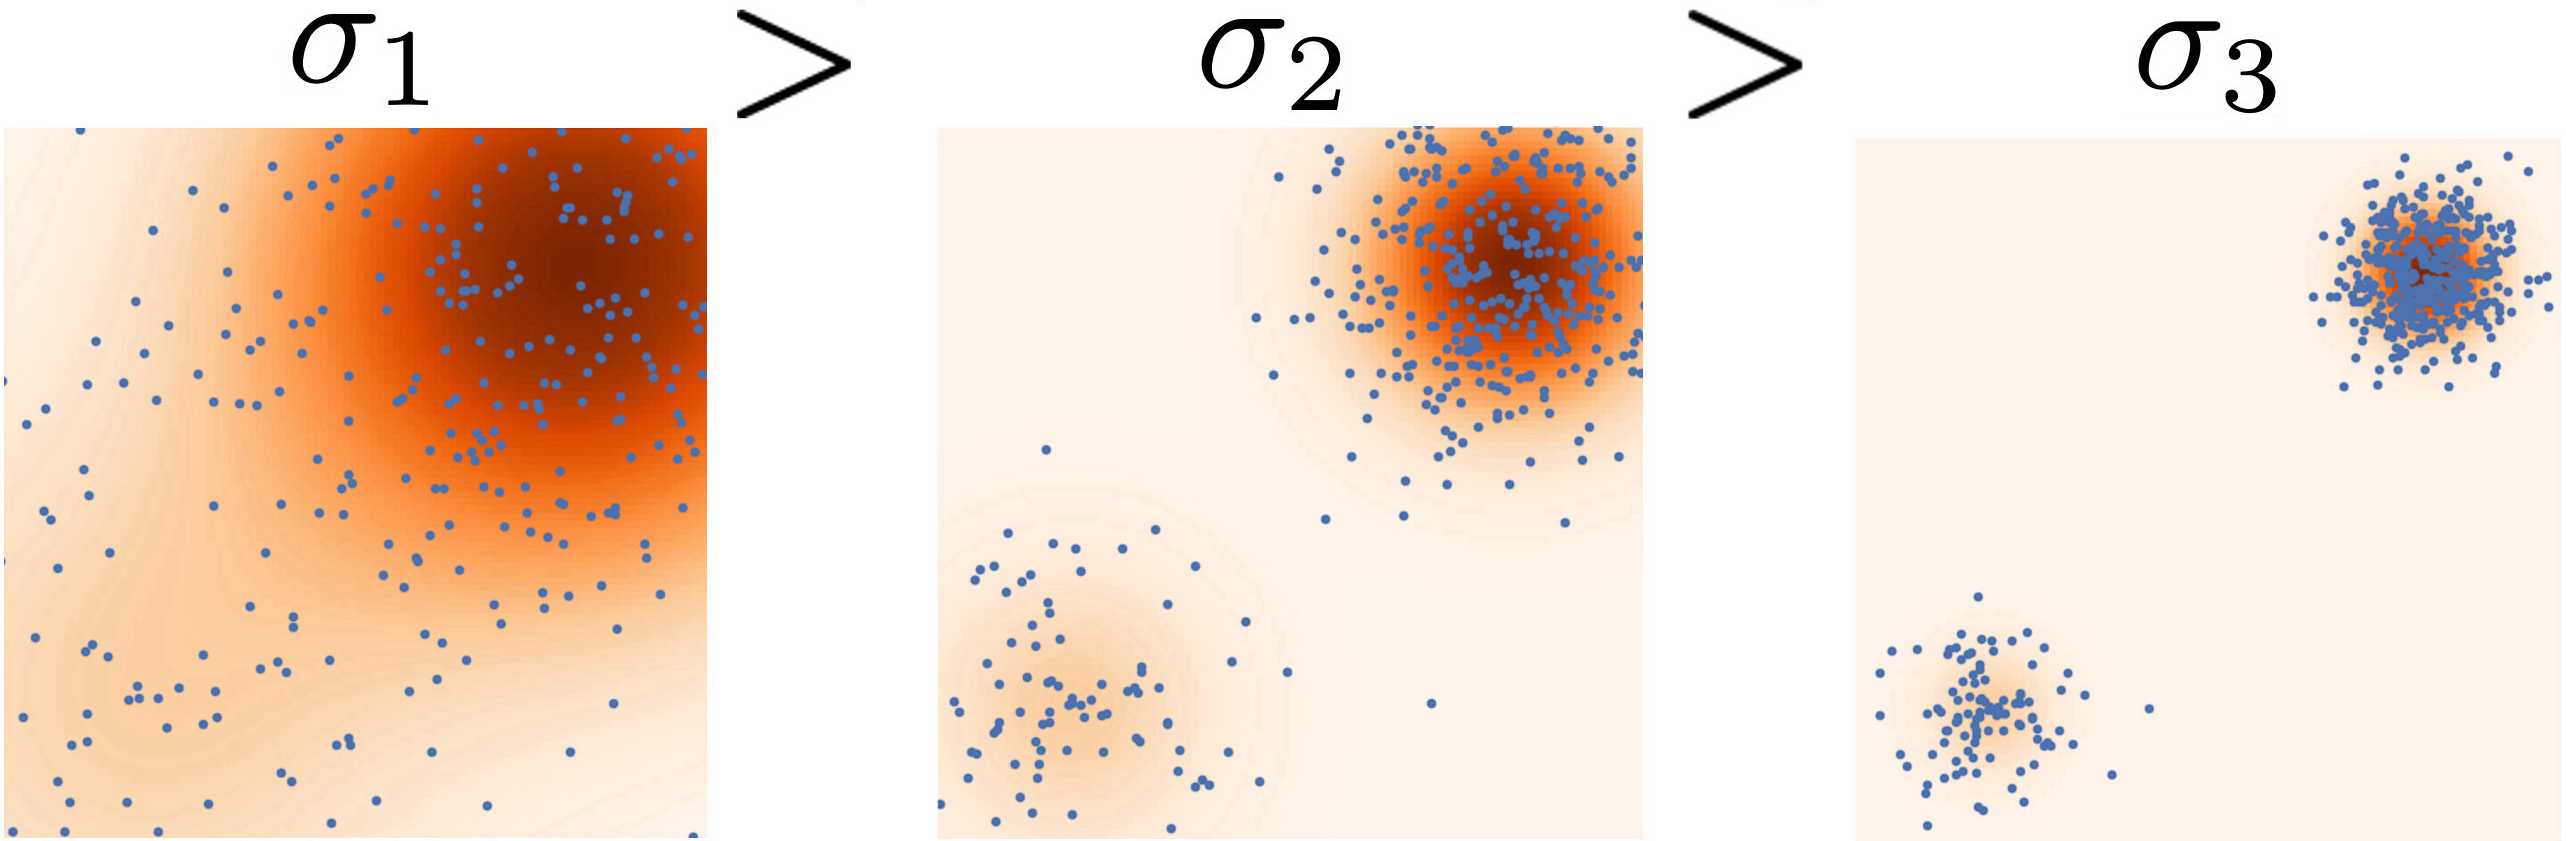
\includegraphics[width=0.55\linewidth]{figs/multi_scale}
	\end{figure}
	\begin{figure}
		
\includegraphics[width=\linewidth]{figs/duoduo}
	\end{figure}
	\myfootnotewithlink{https://arxiv.org/abs/1907.05600}{Song Y. et al. Generative Modeling by Estimating Gradients of the Data Distribution, 2019}
\end{frame}
%=======
\begin{frame}{Recap of previous lecture}
	\vspace{-0.2cm}
	\begin{block}{SDE basics}
		Let define stochastic process $\bx(t)$ with initial condition $\bx(0) \sim p_0(\bx)$:
		\[
			d\bx = \mathbf{f}(\bx, t) dt + g(t) d \bw, 
		\]
		where $\bw(t)$ is the standard Wiener process (Brownian motion)
		\vspace{-0.2cm}
		\[		
			\bw(t) - \bw(s) \sim \cN(0, (t - s) \bI), \quad d \bw = \bepsilon \cdot \sqrt{dt}, \, \text{where } \bepsilon \sim \cN(0, \bI).
		\]
	\end{block}
	\vspace{-0.5cm}
	\begin{block}{Langevin dynamics}
		Let $\bx_0$ be a random vector. Then under mild regularity conditions for small enough $\eta$ samples from the following dynamics
		\vspace{-0.2cm}
		\[
			\bx_{t + 1} = \bx_t + \eta \frac{1}{2} \nabla_{\bx_t} \log p(\bx_t | \btheta) + \sqrt{\eta} \cdot \bepsilon, \quad \bepsilon \sim \cN(0, \bI).
		\]
		will comes from $p(\bx | \btheta)$.
	\end{block}
	The density $p(\bx | \btheta)$ is a \textbf{stationary} distribution for the Langevin SDE.
	\myfootnotewithlink{https://www.stats.ox.ac.uk/~teh/research/compstats/WelTeh2011a.pdf}{Welling M. Bayesian Learning via Stochastic Gradient Langevin Dynamics, 2011}
\end{frame}
%=======
\begin{frame}{Outline}
	\tableofcontents
\end{frame}
%=======
\section{Overview of DDPM}
%=======
\begin{frame}{Denoising diffusion probabilistic model (DDPM)}
	\begin{block}{DDPM is a VAE model}
		\begin{itemize}
			\item Encoder is a fixed Gaussian Markov chain.
			\item Latent variable is a hierarchical (in each step the dim. of the latent equals to the dim of the input).
			\item Decoder is a simple Gaussian model.
			\item Prior distribution is given by parametric Gaussian Makov chain.
		\end{itemize}
	\end{block}
	\begin{minipage}{0.5\linewidth}
		\begin{block}{Forward process}
			\begin{enumerate}
				\item $\bx_0 = \bx \sim \pi(\bx)$;
				\item $\bx_t = \sqrt{1 - \beta} \cdot \bx_{t - 1} + \sqrt{\beta} \cdot \bepsilon$, where $\bepsilon \sim \cN(0, 1)$, $t \geq 1$;
				\item $\bx_T \sim p_{\infty}(\bx) = \cN(0, 1)$.
			\end{enumerate}
		\end{block}
	\end{minipage}%
	\begin{minipage}{0.5\linewidth}
		\begin{block}{Reverse process}
			\begin{enumerate}
				\item $\bx_T \sim p_{\infty}(\bx) = \cN(0, 1)$;
				\item $\bx_{t - 1} = \bsigma_{\btheta}(\bx_t, t) \cdot \bepsilon + \bmu_{\btheta}(\bx_t, t)$;
				\item $\bx_0 = \bx \sim \pi(\bx)$;
			\end{enumerate}
		\end{block}
	\end{minipage}
\end{frame}
%=======
\begin{frame}{Denoising diffusion probabilistic model (DDPM)}
	\begin{block}{Samples}
		\begin{figure}
			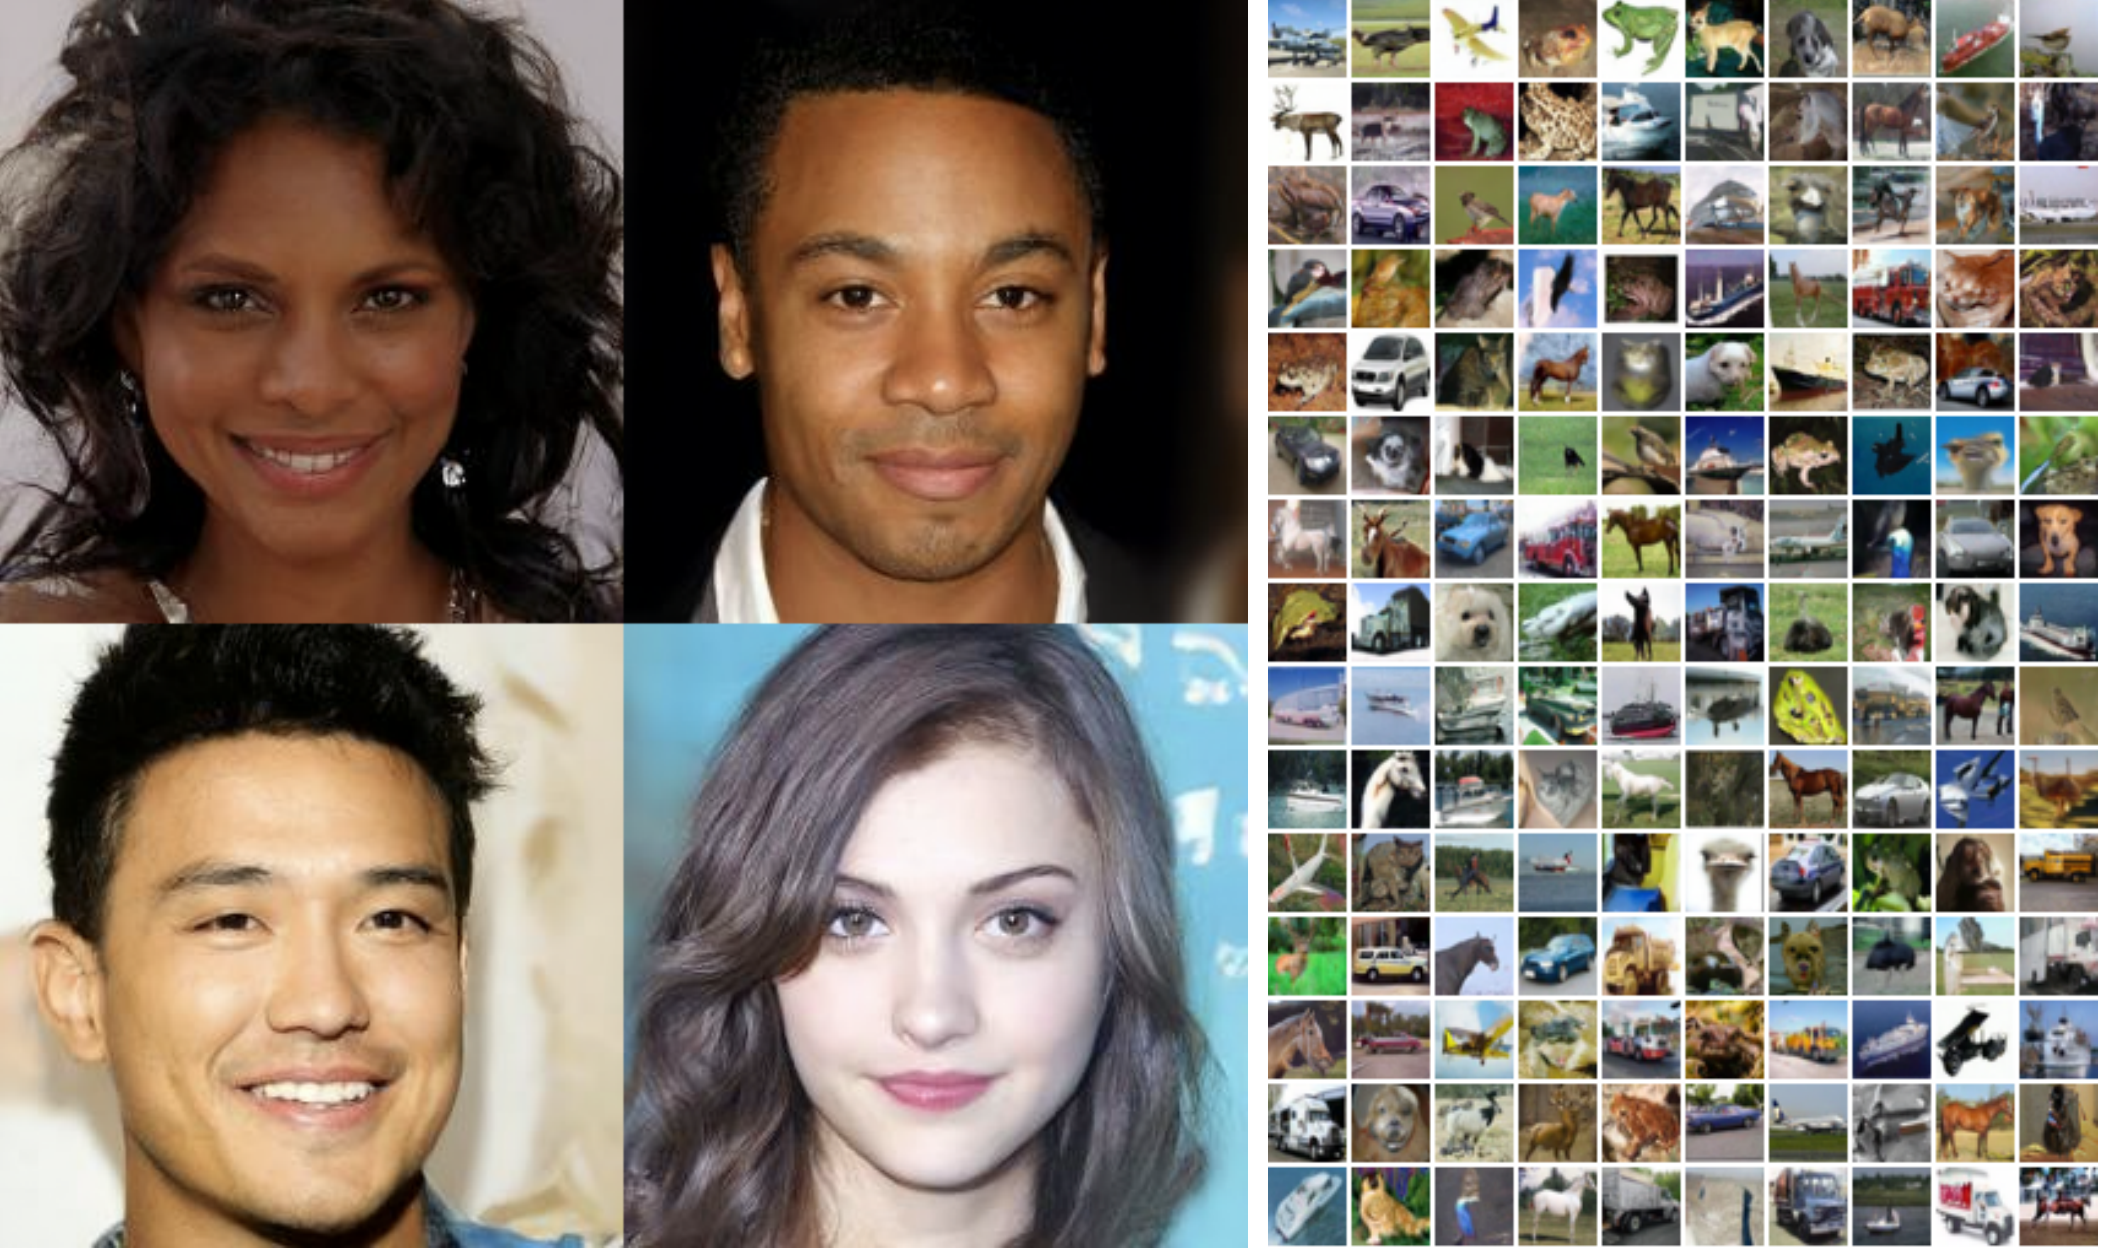
\includegraphics[width=\linewidth]{figs/ddpm_samples}
		\end{figure}
	\end{block}
	\myfootnotewithlink{https://arxiv.org/abs/2006.11239}{Ho J. Denoising Diffusion Probabilistic Models, 2020}
\end{frame}
%=======
\section{Langevin dynamic and SDE basics}
%=======
\begin{frame}{Langevin dynamic}
	Imagine that we have some generative model $p(\bx | \btheta)$.
	\begin{block}{Statement}
		Let $\bx_0$ be a random vector. Then under mild regularity conditions for small enough $\eta$ samples from the following dynamics
		\[
			\bx_{t + 1} = \bx_t + \eta \frac{1}{2} \nabla_{\bx_t} \log p(\bx_t | \btheta) + \sqrt{\eta} \cdot \bepsilon, \quad \bepsilon \sim \cN(0, 1).
		\]
		will comes from $p(\bx | \btheta)$.
	\end{block}
	What do we get if $\bepsilon = \boldsymbol{0}$?
	\begin{block}{Energy-based model}
		\vspace{-0.4cm}
		\[
			p(\bx | \btheta) = \frac{\hat{p}(\bx | \btheta)}{Z_{\btheta}}, \quad \text{where } Z_{\btheta} = \int \hat{p}(\bx | \btheta) d \bx
		\]
		\[
			\nabla_{\bx} \log p(\bx | \btheta) = \nabla_{\bx} \log \hat{p}(\bx | \btheta) - \nabla_{\bx} \log Z_{\btheta} = \nabla_{\bx} \log \hat{p}(\bx | \btheta)
		\]
		Gradient of normalized density equals to gradient of unnormalized density.
	\end{block}
	\myfootnotewithlink{https://www.stats.ox.ac.uk/~teh/research/compstats/WelTeh2011a.pdf}{Welling M. Bayesian Learning via Stochastic Gradient Langevin Dynamics, 2011}
\end{frame}
%=======
\begin{frame}{Stochastic differential equation (SDE)}
	Let define stochastic process $\bx(t)$ with initial condition $\bx(0) \sim p_0(\bx)$:
	\[
		d\bx = \mathbf{f}(\bx, t) dt + g(t) d \bw
	\]
	\vspace{-0.6cm}
	\begin{itemize}
		 \item $\mathbf{f}(\bx, t)$ is the \textbf{drift} function of $\bx(t)$.
		 \item $g(t)$ is the \textbf{diffusion} coefficient of $\bx(t)$.
		 \item If $g(t) = 0$ we get standard ODE.
		 \item $\bw(t)$ is the standard Wiener process (Brownian motion)
		 \[		
		 \bw(t) - \bw(s) \sim \cN(0, t - s), \quad d \bw = \bepsilon \cdot \sqrt{dt}, \, \text{where } \bepsilon \sim \cN(0, 1).
		 \]
	\end{itemize}
	 How to get distribution $p(\bx, t)$ for $\bx(t)$?
 	\begin{block}{Theorem (Kolmogorov-Fokker-Planck)}
 		Evolution of the distribution $p(\bx, t)$ is given by the following ODE:
 		\vspace{-0.2cm}
 		\[
 			\frac{\partial p(\bx, t)}{\partial t} = \text{tr}\left(- \frac{\partial}{\partial \bx} \bigl[ \mathbf{f}(\bx, t) p(\bx, t)\bigr] + \frac{1}{2} g^2(t) \frac{\partial^2 p(\bx, t)}{\partial \bx^2} \right)
 		\]
 		\vspace{-0.6cm}
 	\end{block}
\end{frame}
%=======
\begin{frame}{Langevin SDE (special case)}
	\vspace{-0.4cm}
	\[
		d\bx = {\color{violet}\mathbf{f}(\bx, t)} dt + {\color{teal}g(t)} d \bw, \quad d \bw = \bepsilon \cdot \sqrt{dt}, \quad \bepsilon \sim \cN(0, 1).
	\]
	\vspace{-0.4cm}
	\begin{align*}
		d \bx &= {\color{violet}\frac{1}{2} \frac{\partial}{\partial \bx} \log p(\bx, t)} d t + {\color{teal} 1 }d \bw \\
		\bx_{t + 1} - \bx_t &= \eta \frac{1}{2} \frac{\partial}{\partial \bx} \log p(\bx, t) + \sqrt{\eta} \cdot \bepsilon, \quad \eta \approx dt.
	\end{align*}
	Let apply KFP theorem.
	\begin{multline*}
		\frac{\partial p(\bx, t)}{\partial t} =  \text{tr} \left(- \frac{\partial}{\partial \bx}\left[ {\color{olive}p(\bx, t) \frac{1}{2} \frac{\partial}{\partial \bx} \log p(\bx, t)} \right]  + \frac{1}{2} \frac{\partial^2 p(\bx, t)}{\partial \bx^2} \right) = \\
		= \text{tr} \left(- \frac{\partial}{\partial \bx}\left[ {\color{olive}\frac{1}{2} \frac{\partial}{\partial \bx} p(\bx, t) } \right]  + \frac{1}{2} \frac{\partial^2 p(\bx, t)}{\partial \bx^2} \right) = 0
	\end{multline*}
	The density $p(\bx, t) = \text{const}$.
	\begin{block}{Langevin dynamic}
		\vspace{-0.3cm}
		\[
			\bx_{t + 1} = \bx_t + \eta \frac{1}{2} \nabla_{\bx} \log p(\bx | \btheta) + \sqrt{\eta} \cdot \bepsilon, \quad \eta \approx dt.
		\]
		\vspace{-0.3cm}
	\end{block}
\end{frame}
%=======
\begin{frame}{Stochastic differential equation (SDE)}
	\vspace{-0.4cm}
	\begin{block}{Statement}
		Let $\bx_0$ be a random vector. Then samples from the following dynamics
		\[
			\bx_{t + 1} = \bx_t + \eta \frac{1}{2} \nabla_{\bx_t} \log p(\bx_t | \btheta) + \sqrt{\eta} \cdot \bepsilon, \quad \bepsilon \sim \cN(0, 1).
		\]
		will come from $p(\bx | \btheta)$ under mild regularity conditions for small enough $\eta$ and large enough $t$.
	\end{block}
	\begin{minipage}{0.6\linewidth}
		The density $p(\bx | \btheta)$ is a \textbf{stationary} distribution for this SDE.
	\end{minipage}%
	\begin{minipage}{0.35\linewidth}
		\vspace{-0.2cm}
		\begin{figure}
			\centering
			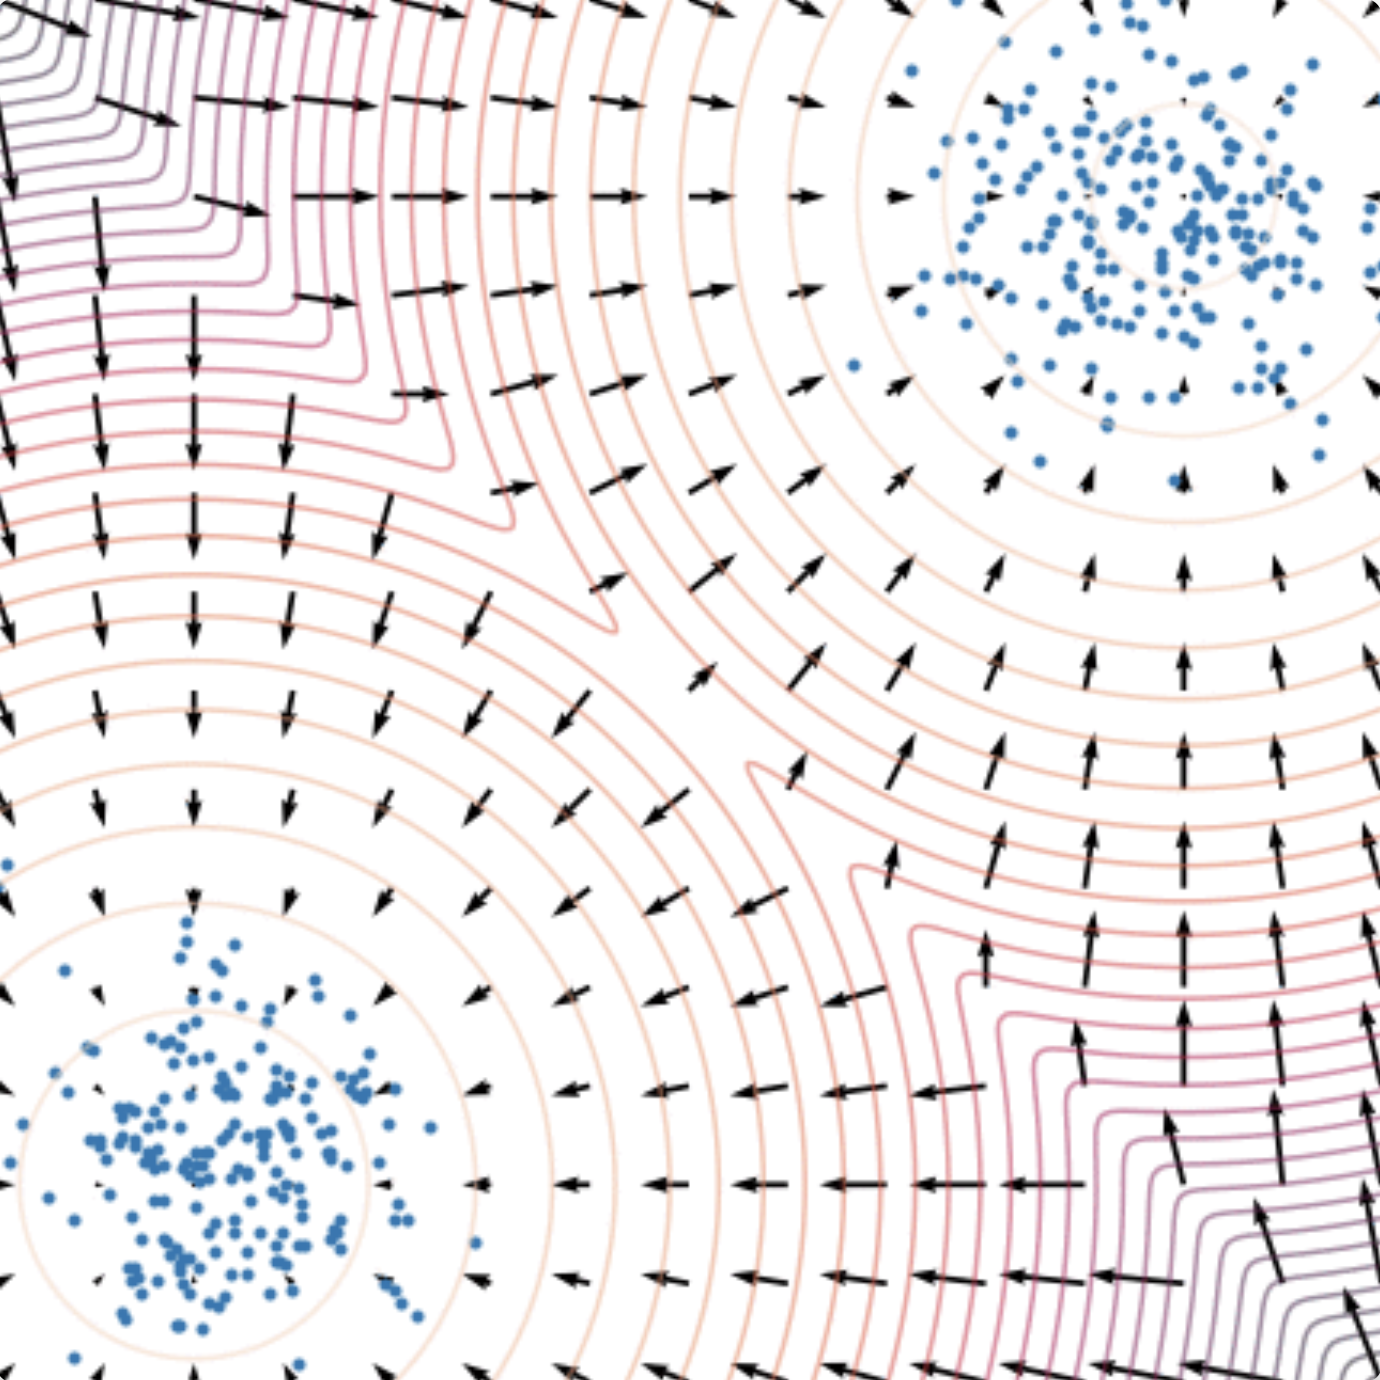
\includegraphics[width=0.9\linewidth]{figs/langevin_dynamic}
		\end{figure}
	\end{minipage}
	\myfootnotewithlink{https://yang-song.github.io/blog/2021/score/}{Song Y. Generative Modeling by Estimating Gradients of the Data Distribution, blog post, 2021} 
	\end{frame}
%=======
\section{Score matching}
%=======
\begin{frame}{Score matching}
	We could sample from the model using Langevin dynamics if we have $\nabla_{\bx}\log p(\bx| \btheta)$.
	\begin{block}{Fisher divergence}
		\vspace{-0.3cm}
		\[
		D_F(\pi, p) = \frac{1}{2}\bbE_{\pi}\bigl\| \nabla_{\bx}\log p(\bx| \btheta) - \nabla_\bx \log \pi(\bx) \bigr\|^2_2 \rightarrow \min_{\btheta}
		\]
		\vspace{-0.5cm}
	\end{block}
	Let introduce \textbf{score function} $\bs_{\btheta}(\bx) = \nabla_{\bx}\log p(\bx| \btheta)$. 
	\vspace{-0.2cm}
	\begin{figure}
		\centering
		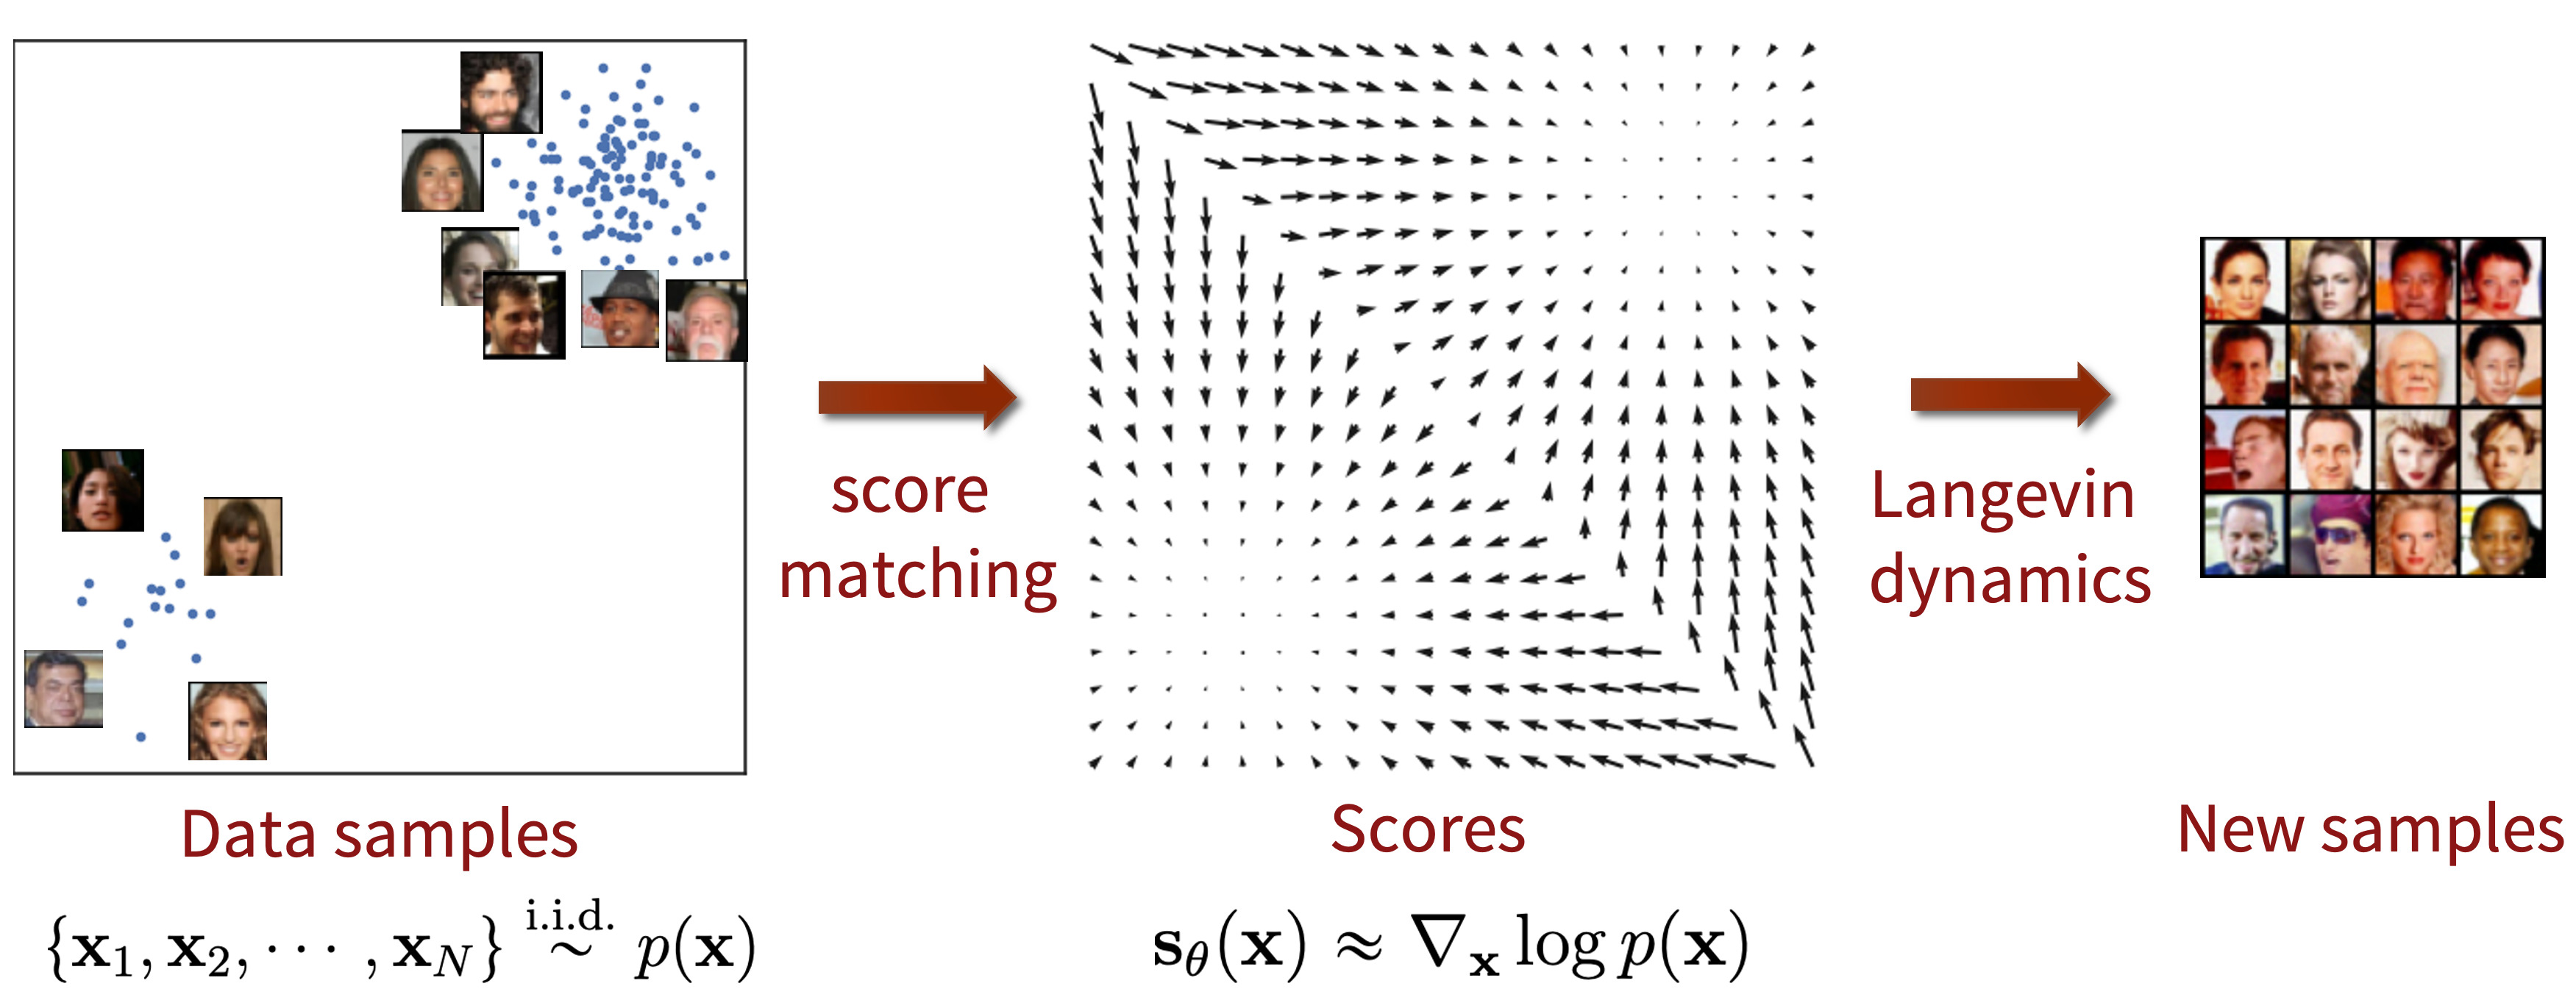
\includegraphics[width=0.75\linewidth]{figs/smld}
	\end{figure}
	\vspace{-0.3cm} 
	\textbf{Problem:} we do not know $\nabla_\bx \log \pi(\bx)$.
	\myfootnotewithlink{https://yang-song.github.io/blog/2021/score/}{Song Y. Generative Modeling by Estimating Gradients of the Data Distribution, blog post, 2021}
\end{frame}
%=======
\begin{frame}{Score matching}
	\begin{block}{Theorem (implicit score matching)}
		Under some regularity conditions, it holds
		\vspace{-0.2cm}
		\[
		\frac{1}{2} \bbE_{\pi}\bigl\| \bs_{\btheta}(\bx) - \nabla_\bx \log \pi(\bx) \bigr\|^2_2 = \bbE_{\pi}\Bigr[ \frac{1}{2}\| \bs_{\btheta}(\bx) \|_2^2 + \text{tr}\bigl(\nabla_{\bx} \bs_{\btheta}(\bx)\bigr) \Bigr] + \text{const}
		\]
		\vspace{-0.6cm}
	\end{block}
	\begin{block}{Proof (only for 1D)}
		\vspace{-0.6cm}
		{\small
			\begin{multline*}
				\bbE_{\pi}\bigl\| s(x) - \nabla_x \log \pi(x) \bigr\|^2_2 = \bbE_{\pi} \bigl[ s(x)^2 + (\nabla_x \log \pi(x))^2 - 2{\color{teal}[s(x) \nabla_x \log \pi(x) ] \bigr] }
			\end{multline*}
			\vspace{-0.8cm}
			\begin{align*}
				{\color{teal}\bbE_{\pi} [{\color{violet}s(x) } \nabla_x \log \pi(x) ] } &= \int {\color{olive}\pi(x) {\color{violet}\nabla_x \log p(x)} \nabla_x \log \pi(x)} d x \\ 
				&= \int {\color{violet}\nabla_x \log p(x) } {\color{olive}\nabla_x \pi(x) } dx = \Bigl.\pi(x) \nabla_x \log p(x) \Bigr|_{-\infty}^{+\infty} \\
				&- \int \nabla^2_x \log p(x)  \pi(x) dx =- \bbE_{\pi} \nabla^2_x \log p(x) =- \bbE_{\pi} \nabla_x s(x)
			\end{align*}
			\[
			\frac{1}{2} \bbE_{\pi}\bigl\| s(x) - \nabla_x \log \pi(x) \bigr\|^2_2 = \bbE_{\pi} \Bigr[\frac{1}{2} s(x)^2 + \nabla_x s(x) \Bigl]+ \text{const}.
			\]
		}
	\end{block}
	\myfootnotewithlink{https://jmlr.org/papers/volume6/hyvarinen05a/old.pdf}{Hyvarinen A. Estimation of non-normalized statistical models by score matching, 2005} 
\end{frame}
%=======
\begin{frame}{Score matching}
	\vspace{-0.3cm}
	\begin{block}{Theorem (implicit score matching)}
		\vspace{-0.6cm}
		\[
		{\color{violet}\frac{1}{2} \bbE_{\pi}\bigl\| \bs_{\btheta}(\bx) - \nabla_\bx \log \pi(\bx) \bigr\|^2_2} = {\color{teal}\bbE_{\pi}\Bigr[ \frac{1}{2}\| \bs_{\btheta}(\bx) \|_2^2 + \text{tr}\bigl(\nabla_{\bx} \bs_{\btheta}(\bx)\bigr) \Bigr]} + \text{const}
		\]
		Here $\nabla_{\bx} \bs_{\btheta}(\bx) = \nabla_{\bx}^2 \log p(\bx | \btheta)$ is a Hessian matrix.
	\end{block}
	\begin{enumerate}
		\item {\color{violet}The left hand side} is intractable due to unknown $\pi(\bx)$ -- \textbf{denoising score matching}. 
		\item {\color{teal}The right hand side} is complex due to Hessian matrix -- \textbf{sliced score matching}.
	\end{enumerate}
	\begin{block}{Sliced score matching (Hutchinson's trace estimation)}
	\vspace{-0.3cm}
	\[
		\text{tr}\bigl(\nabla_{\bx} \bs_{\btheta}(\bx)\bigr) = \mathbb{E}_{p(\bepsilon)} \left[ {\color{olive}\bepsilon^T \nabla_{\bx} \bs_{\btheta}(\bx)} \bepsilon \right]
	\]
	\end{block}
	\myfootnote{\href{https://yang-song.net/blog/2021/ssm/}{Song Y. Sliced Score Matching: A Scalable Approach to Density and Score Estimation, 2019} \\
	\href{https://yang-song.net/blog/2021/score/}{Song Y. Generative Modeling by Estimating Gradients of the Data Distribution, blog post, 2021}}
\end{frame}
%=======
\begin{frame}{Denoising score matching}
	Let perturb original data $\bx \sim \pi(\bx)$ by random normal noise 
	\[
		\bx' = \bx + \sigma \cdot \bepsilon, \quad \bepsilon \sim \cN(0, 1), \quad p(\bx' | \bx, \sigma) = \cN(\bx' | \bx, \sigma^2 \bI)
	\]
	\vspace{-0.4cm}
	\[
		\pi(\bx' | \sigma) = \int \pi(\bx) p(\bx' | \bx, \sigma) d\bx.
	\]
	\vspace{-0.4cm} \\
	Then the solution of 
	\[
		\frac{1}{2} \bbE_{\pi(\bx' | \sigma)}\bigl\| \bs_{\btheta}(\bx', \sigma) - \nabla_{\bx'} \log \pi(\bx' | \sigma) \bigr\|^2_2 \rightarrow \min_{\btheta}
	\]
	\vspace{-0.3cm} \\
	satisfies $\bs_{\btheta}(\bx', \sigma) \approx \bs_{\btheta}(\bx', 0) = \bs_{\btheta}(\bx)$ if $\sigma$ is small enough.
	\myfootnotewithlink{http://www.iro.umontreal.ca/~vincentp/Publications/smdae_techreport.pdf}{Vincent P. A Connection Between Score Matching and Denoising Autoencoders, 2010}
\end{frame}
%=======
\begin{frame}{Denoising score matching}
	\begin{block}{Theorem}
	\vspace{-0.5cm}
	\begin{multline*}
		\bbE_{\pi(\bx' | \sigma)}\bigl\| \bs_{\btheta}(\bx', \sigma) - \nabla_{\bx'} \log \pi(\bx' | \sigma) \bigr\|^2_2 = \\ = \bbE_{\pi(\bx)} \bbE_{p(\bx' | \bx, \sigma)}\bigl\| \bs_{\btheta}(\bx', \sigma) - \nabla_{\bx'} \log p(\bx' | \bx, \sigma) \bigr\|^2_2 + \text{const}(\btheta)
	\end{multline*}
	\vspace{-0.5cm}
	\end{block}
	\begin{block}{Gradient of the noise kernel}
	\vspace{-0.3cm}
	\[
		\nabla_{\bx'} \log p(\bx' | \bx, \sigma) = \nabla_{\bx'} \log \cN(\bx' | \bx, \sigma^2 \bI) = - \frac{\bx' - \bx}{\sigma^2}
	\]
	\vspace{-0.3cm}
	\end{block}
	\begin{itemize}
		\item The RHS does not need to compute $\nabla_{\bx'} \log \pi(\bx' | \sigma)$ and even $\nabla_{\bx'} \log \pi(\bx')$.
		\item $\bs_{\btheta}(\bx', \sigma)$ tries to \textbf{denoise} a corrupted sample $\bx'$.
		\item Score function $\bs_{\btheta}(\bx', \sigma)$ parametrized by $\sigma$. How to make it?
	\end{itemize}
	\myfootnotewithlink{http://www.iro.umontreal.ca/~vincentp/Publications/smdae_techreport.pdf}{Vincent P. A Connection Between Score Matching and Denoising Autoencoders, 2010}
\end{frame}
%=======
\section{Noise conditioned score network}
%=======
\begin{frame}{Denoising score matching}
	\begin{itemize}
		\item If $\sigma$ is \textbf{small}, the score function is not accurate and Langevin dynamics will probably fail to jump between modes.
		\begin{figure}
			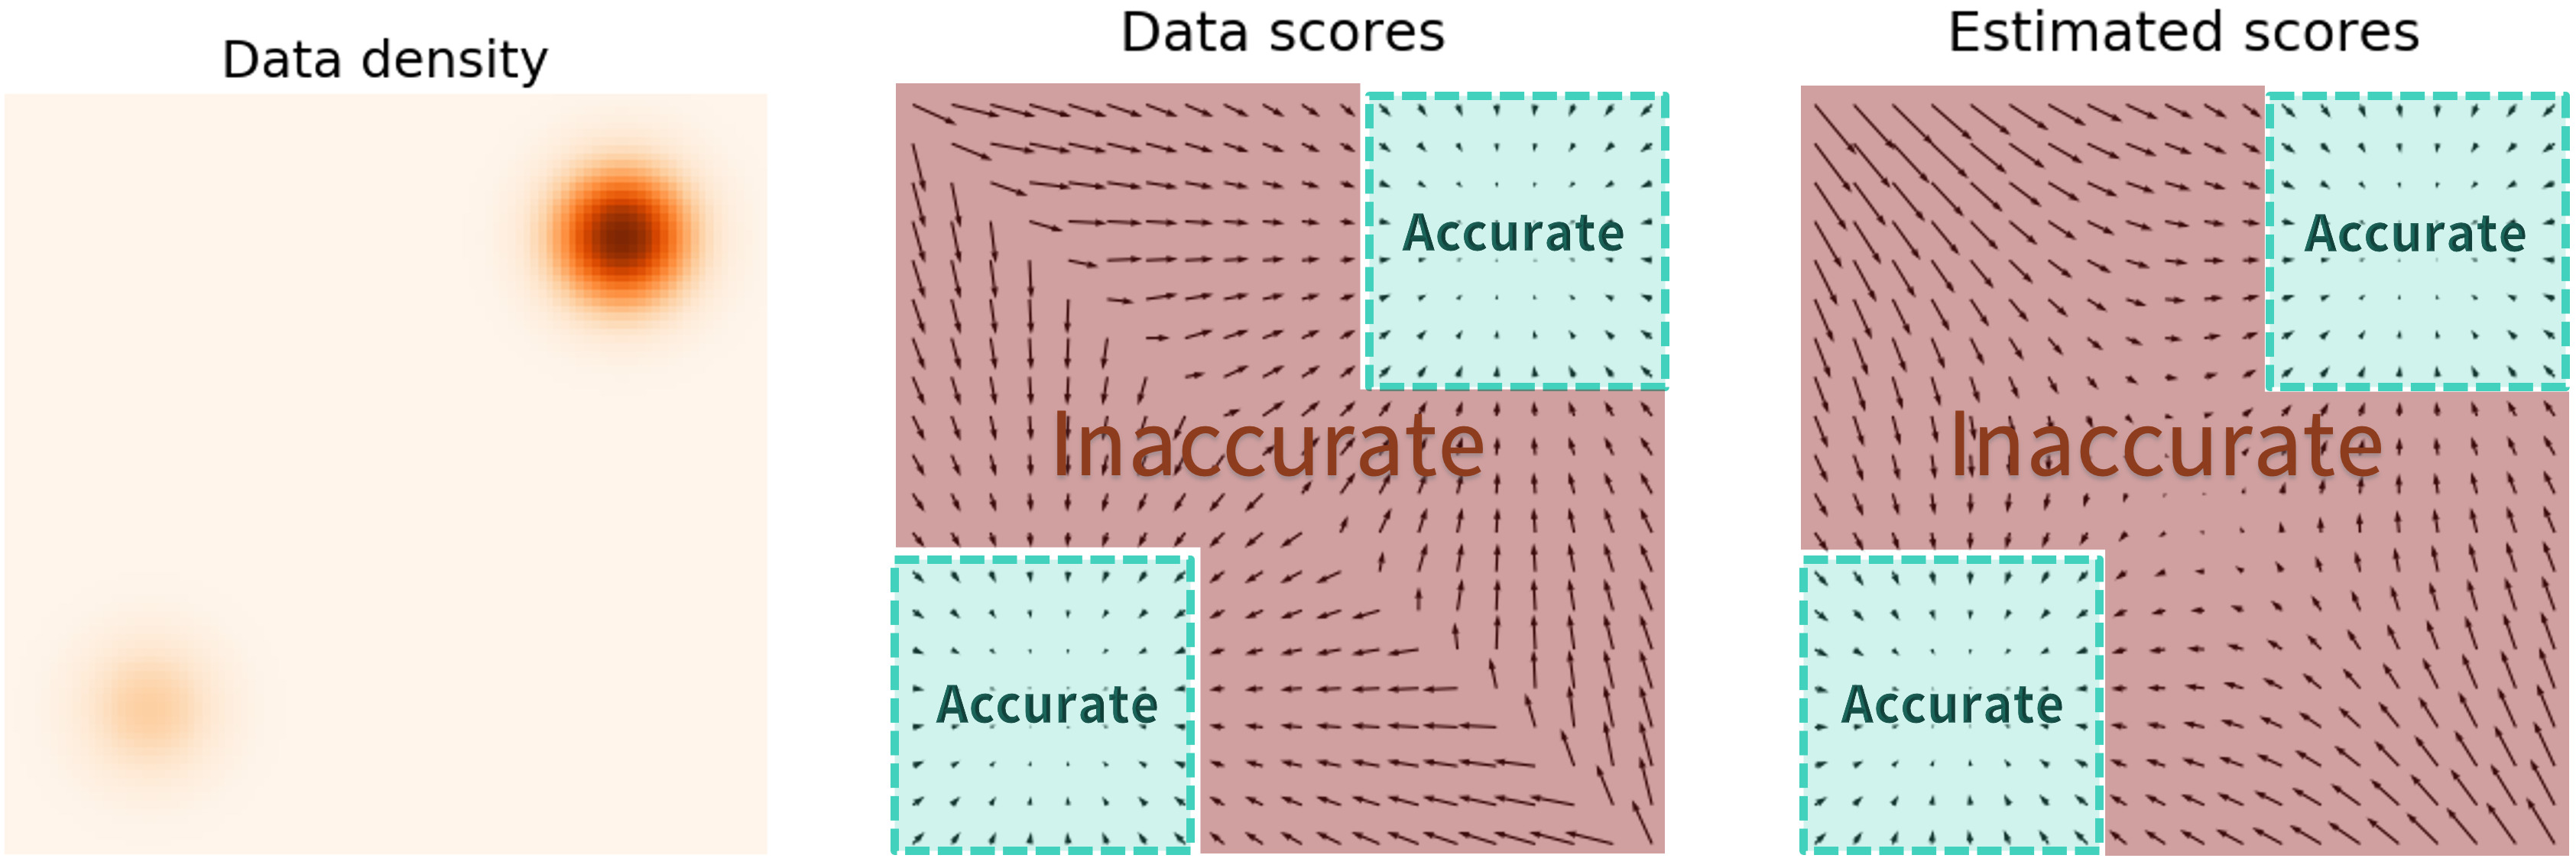
\includegraphics[width=0.75\linewidth]{figs/pitfalls}
		\end{figure}
		\item If $\sigma$ is \textbf{large}, it is good for low-density regions and  multimodal distributions, but we will learn too corrupted distribution.
		\begin{figure}
			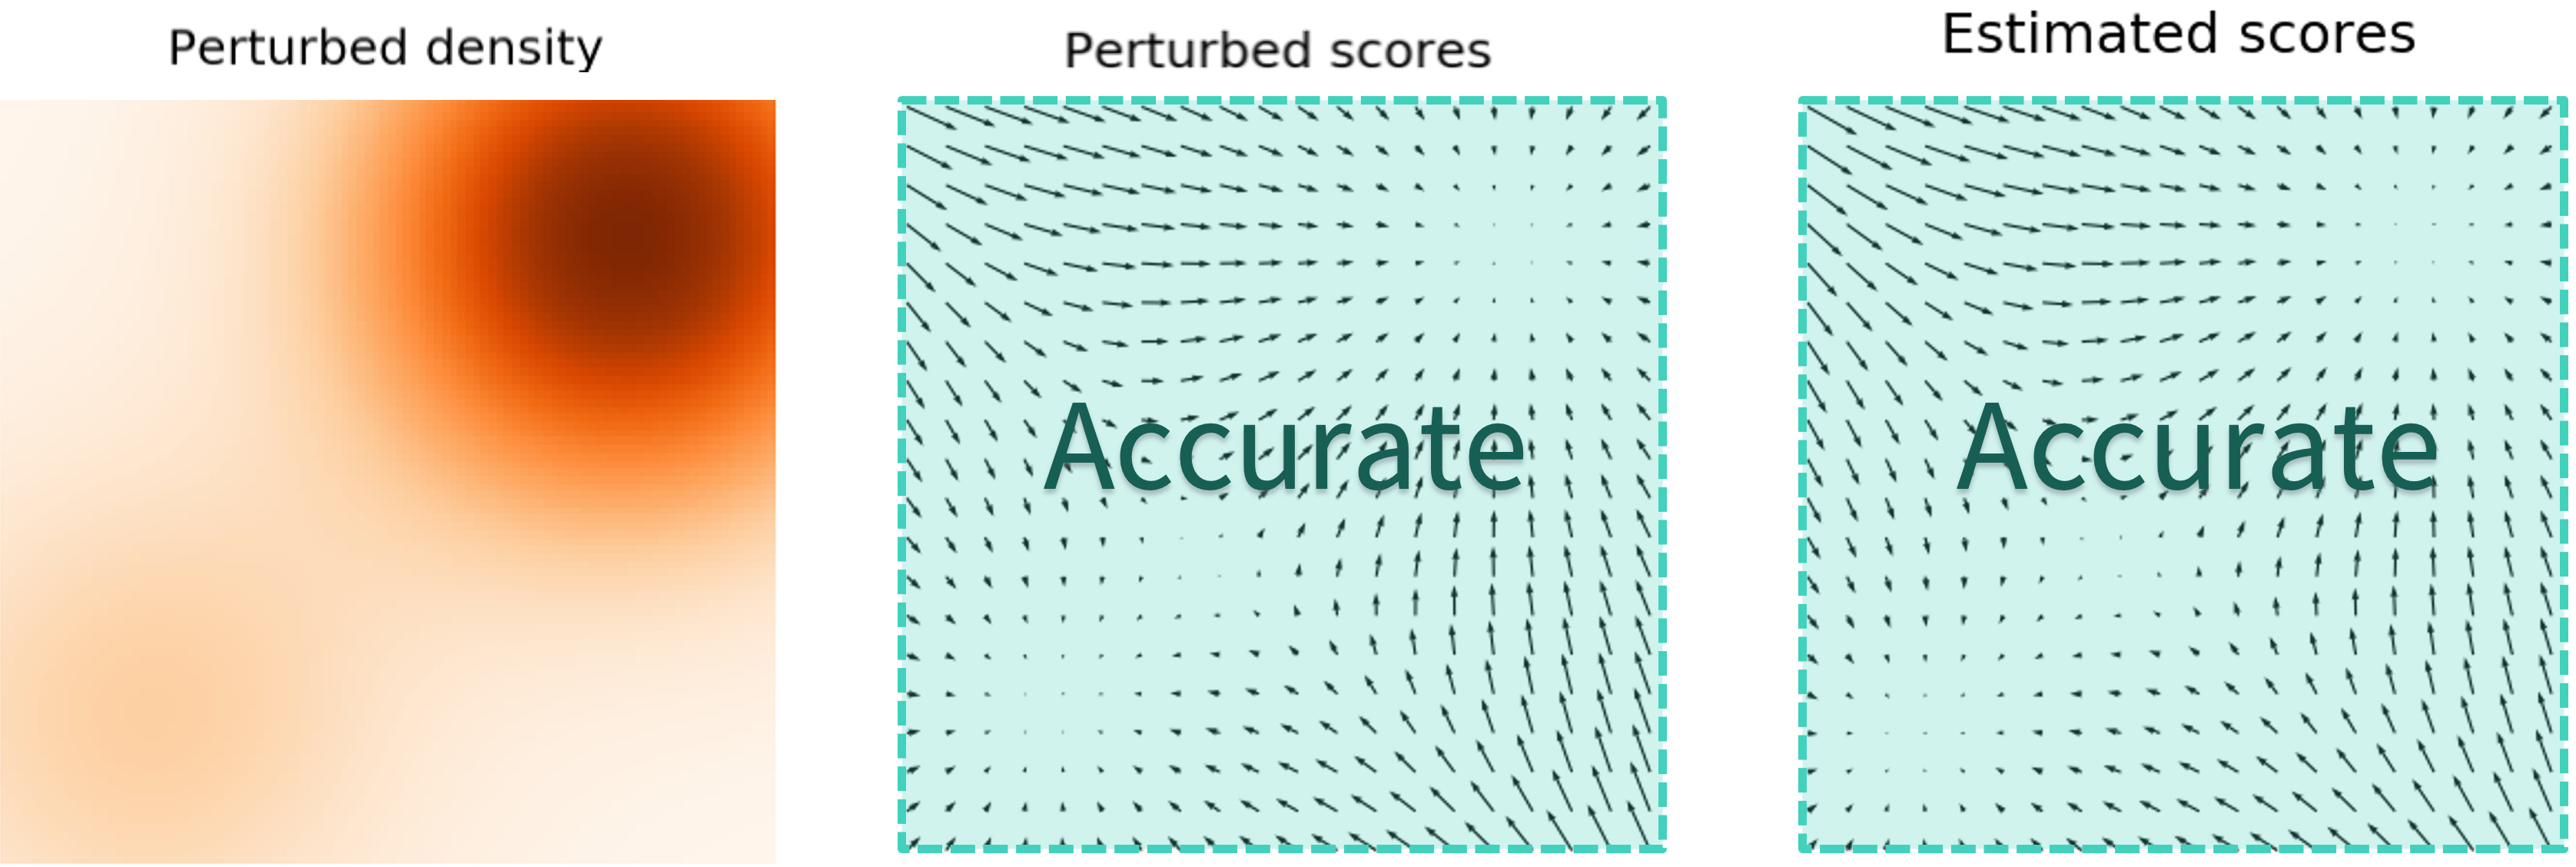
\includegraphics[width=0.75\linewidth]{figs/single_noise}
		\end{figure}
	\end{itemize}
	\myfootnotewithlink{https://yang-song.github.io/blog/2021/score/}{Song Y. Generative Modeling by Estimating Gradients of the Data Distribution, blog post, 2021}
\end{frame}
%=======
\begin{frame}{Noise conditioned score network}
	\begin{itemize}
		\item Define the sequence of noise levels: $\sigma_1 > \sigma_2 > \dots > \sigma_L$.
		\item Perturb the original data with the different noise level to get $\pi(\bx' | \sigma_1), \dots, \pi(\bx' | \sigma_L)$.
		\item Train denoised score function $\bs_{\btheta}(\bx', \sigma)$ for each noise level:
		\vspace{-0.2cm}
		\[
			\sum_{l=1}^L {\color{violet}\sigma_l^2} \bbE_{\pi(\bx)} \bbE_{p(\bx' | \bx, \sigma_l)}\bigl\| \bs_{\btheta}(\bx', \sigma_l) - \nabla_\bx' \log p(\bx' | \bx, \sigma_l) \bigr\|^2_2 \rightarrow \min_{\btheta}
		\]
		\item Sample from \textbf{annealed} Langevin dynamics (for $l=1, \dots, L$).
	\end{itemize}
	\begin{figure}
		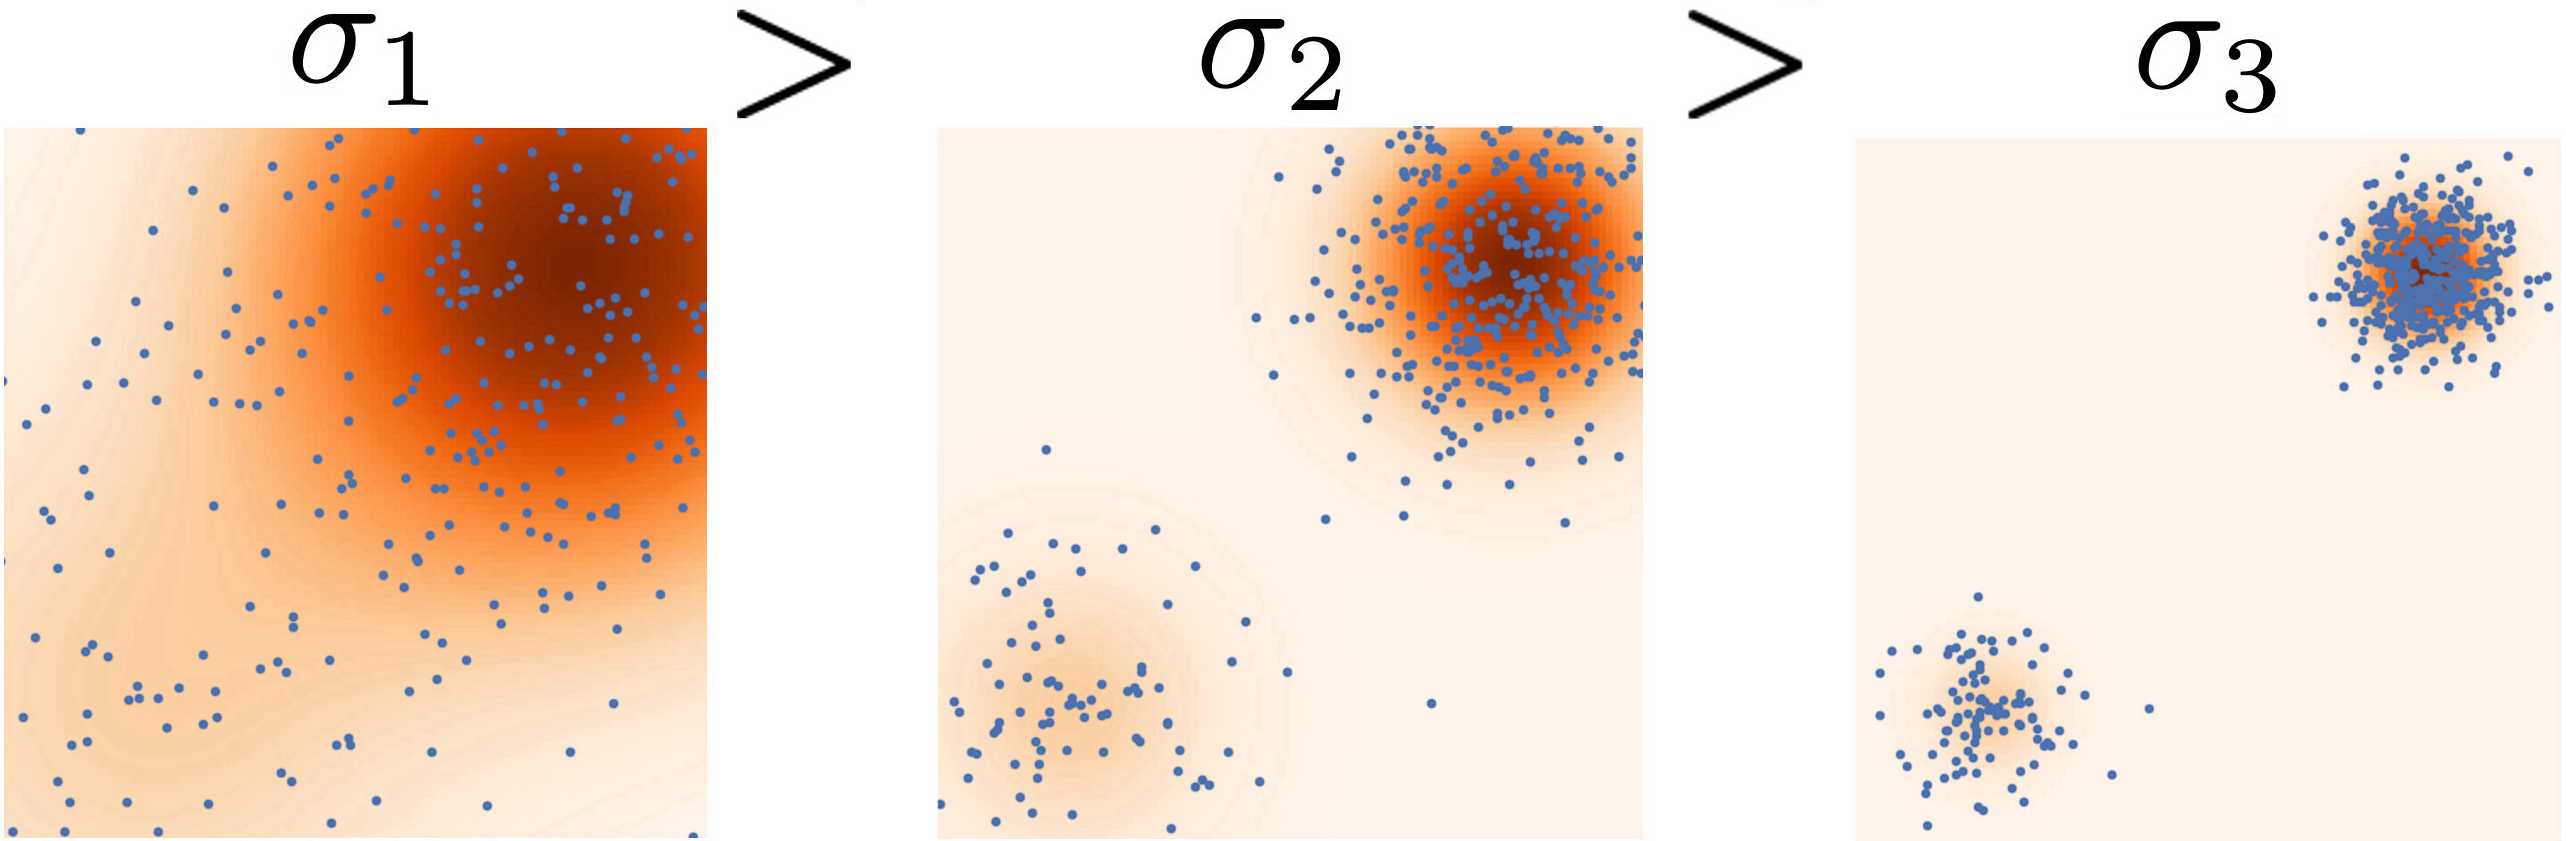
\includegraphics[width=0.6\linewidth]{figs/multi_scale}
	\end{figure}
	\begin{figure}
		
\includegraphics[width=\linewidth]{figs/duoduo}
	\end{figure}
	\myfootnotewithlink{https://arxiv.org/abs/1907.05600}{Song Y. et al. Generative Modeling by Estimating Gradients of the Data Distribution, 2019}
\end{frame}
%=======
\begin{frame}{Noise conditioned score network}
	\begin{minipage}{0.5\linewidth}
		\vspace{-0.7cm}
		\begin{block}{Training: loss function}
			\vspace{-0.8cm}
			\[
			\sum_{i=1}^L \sigma_l^2\bbE_{\pi(\bx)} \bbE_{\bepsilon}\left\| \bs_l + \frac{\bepsilon}{\sigma_l} \right\|^2_2,
			\]
		\end{block}
		\vspace{-0.5cm}
		Here
		\begin{itemize}
			\item $\bs_l = \bs_{\btheta}(\bx + \sigma_l \cdot \bepsilon, \sigma_l)$.
			\item $\nabla_{\bx'} \log p(\bx' | \bx, \sigma) = - \frac{\bx' - \bx}{\sigma^2} = - \frac{\bepsilon}{\sigma_l}$.
		\end{itemize}
	\end{minipage}%
	\begin{minipage}{0.5\linewidth}
		\begin{block}{Inference: annealed Langevin dynamic}
			\begin{figure}
				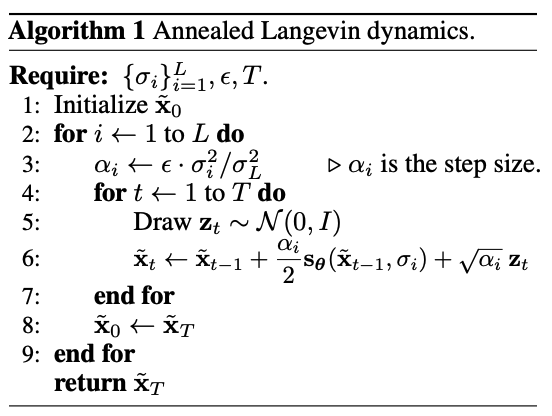
\includegraphics[width=0.9\linewidth]{figs/ald}
			\end{figure}
		\end{block}
	\end{minipage}
	\vspace{-0.7cm}
	\begin{block}{Samples}
		\begin{figure}
			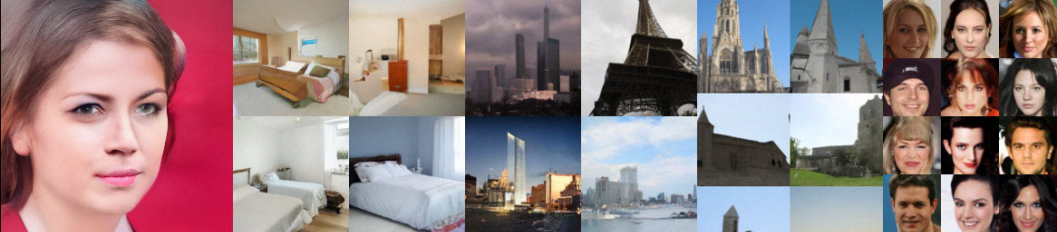
\includegraphics[width=\linewidth]{figs/NCSNv2}
		\end{figure}
	\end{block}
	\myfootnotewithlink{https://arxiv.org/abs/2006.09011}{Song Y. et al. Improved Techniques for Training Score-Based Generative Models, 2020}
\end{frame}
%=======
\begin{frame}{Gaussian diffusion model vs Score matching}
	\vspace{-0.3cm}
	\[
		\cL_t = {\color{olive}\bbE_{\bepsilon}} \left[ \frac{\beta_t^2}{2\tilde{\beta}_t (1 - \beta_t)} \left\| {\color{violet}\frac{\bepsilon}{\sqrt{1 - \bar{\alpha}_t}}} - {\color{teal}\frac{\bepsilon_{\btheta}(\bx_t, t)}{\sqrt{1 - \bar{\alpha}_t}}}\right\|^2 \right]
	\]
	\begin{itemize}
		\item Result from Statement 2
		\[
			q(\bx_t | \bx_0) = \cN(\bx_t | \sqrt{\bar{\alpha}_t} \cdot \bx_0, (1 - \bar{\alpha}_t) \cdot \bI).
		\]
		\item Score of noised distribution
		\[
			\nabla_{\bx_t} \log q(\bx_t | \bx_0) = - \frac{\bepsilon}{\sqrt{1 - \bar{\alpha}_t}}, \quad \text{where } \bepsilon \sim \cN(0, 1).
		\]
		\item Let reparametrize our model: 
		\[
			\bs_{\btheta}(\bx_t, t) = - \frac{\bepsilon_{\btheta}(\bx_t, t)}{\sqrt{1 - \bar{\alpha}_t}}.
		\]
	\end{itemize}
	\begin{block}{Noise conditioned score network}
		\vspace{-0.2cm}
		\[
			{\color{olive}\bbE_{p(\bx' | \bx, \sigma_l)}}\bigl\| {\color{teal}\bs(\bx', \btheta, \sigma_l)} - {\color{violet}\nabla_{\bx'} \log p(\bx' | \bx, \sigma_l)} \bigr\|^2_2 \rightarrow \min_{\btheta}
		\]
	\end{block}
	\myfootnotewithlink{https://arxiv.org/abs/2006.11239}{Ho J. Denoising Diffusion Probabilistic Models, 2020}
	\end{frame}
%=======
\section{The worst course overview}
%=======
\begin{frame}{The worst course overview :)}
	\begin{figure}
		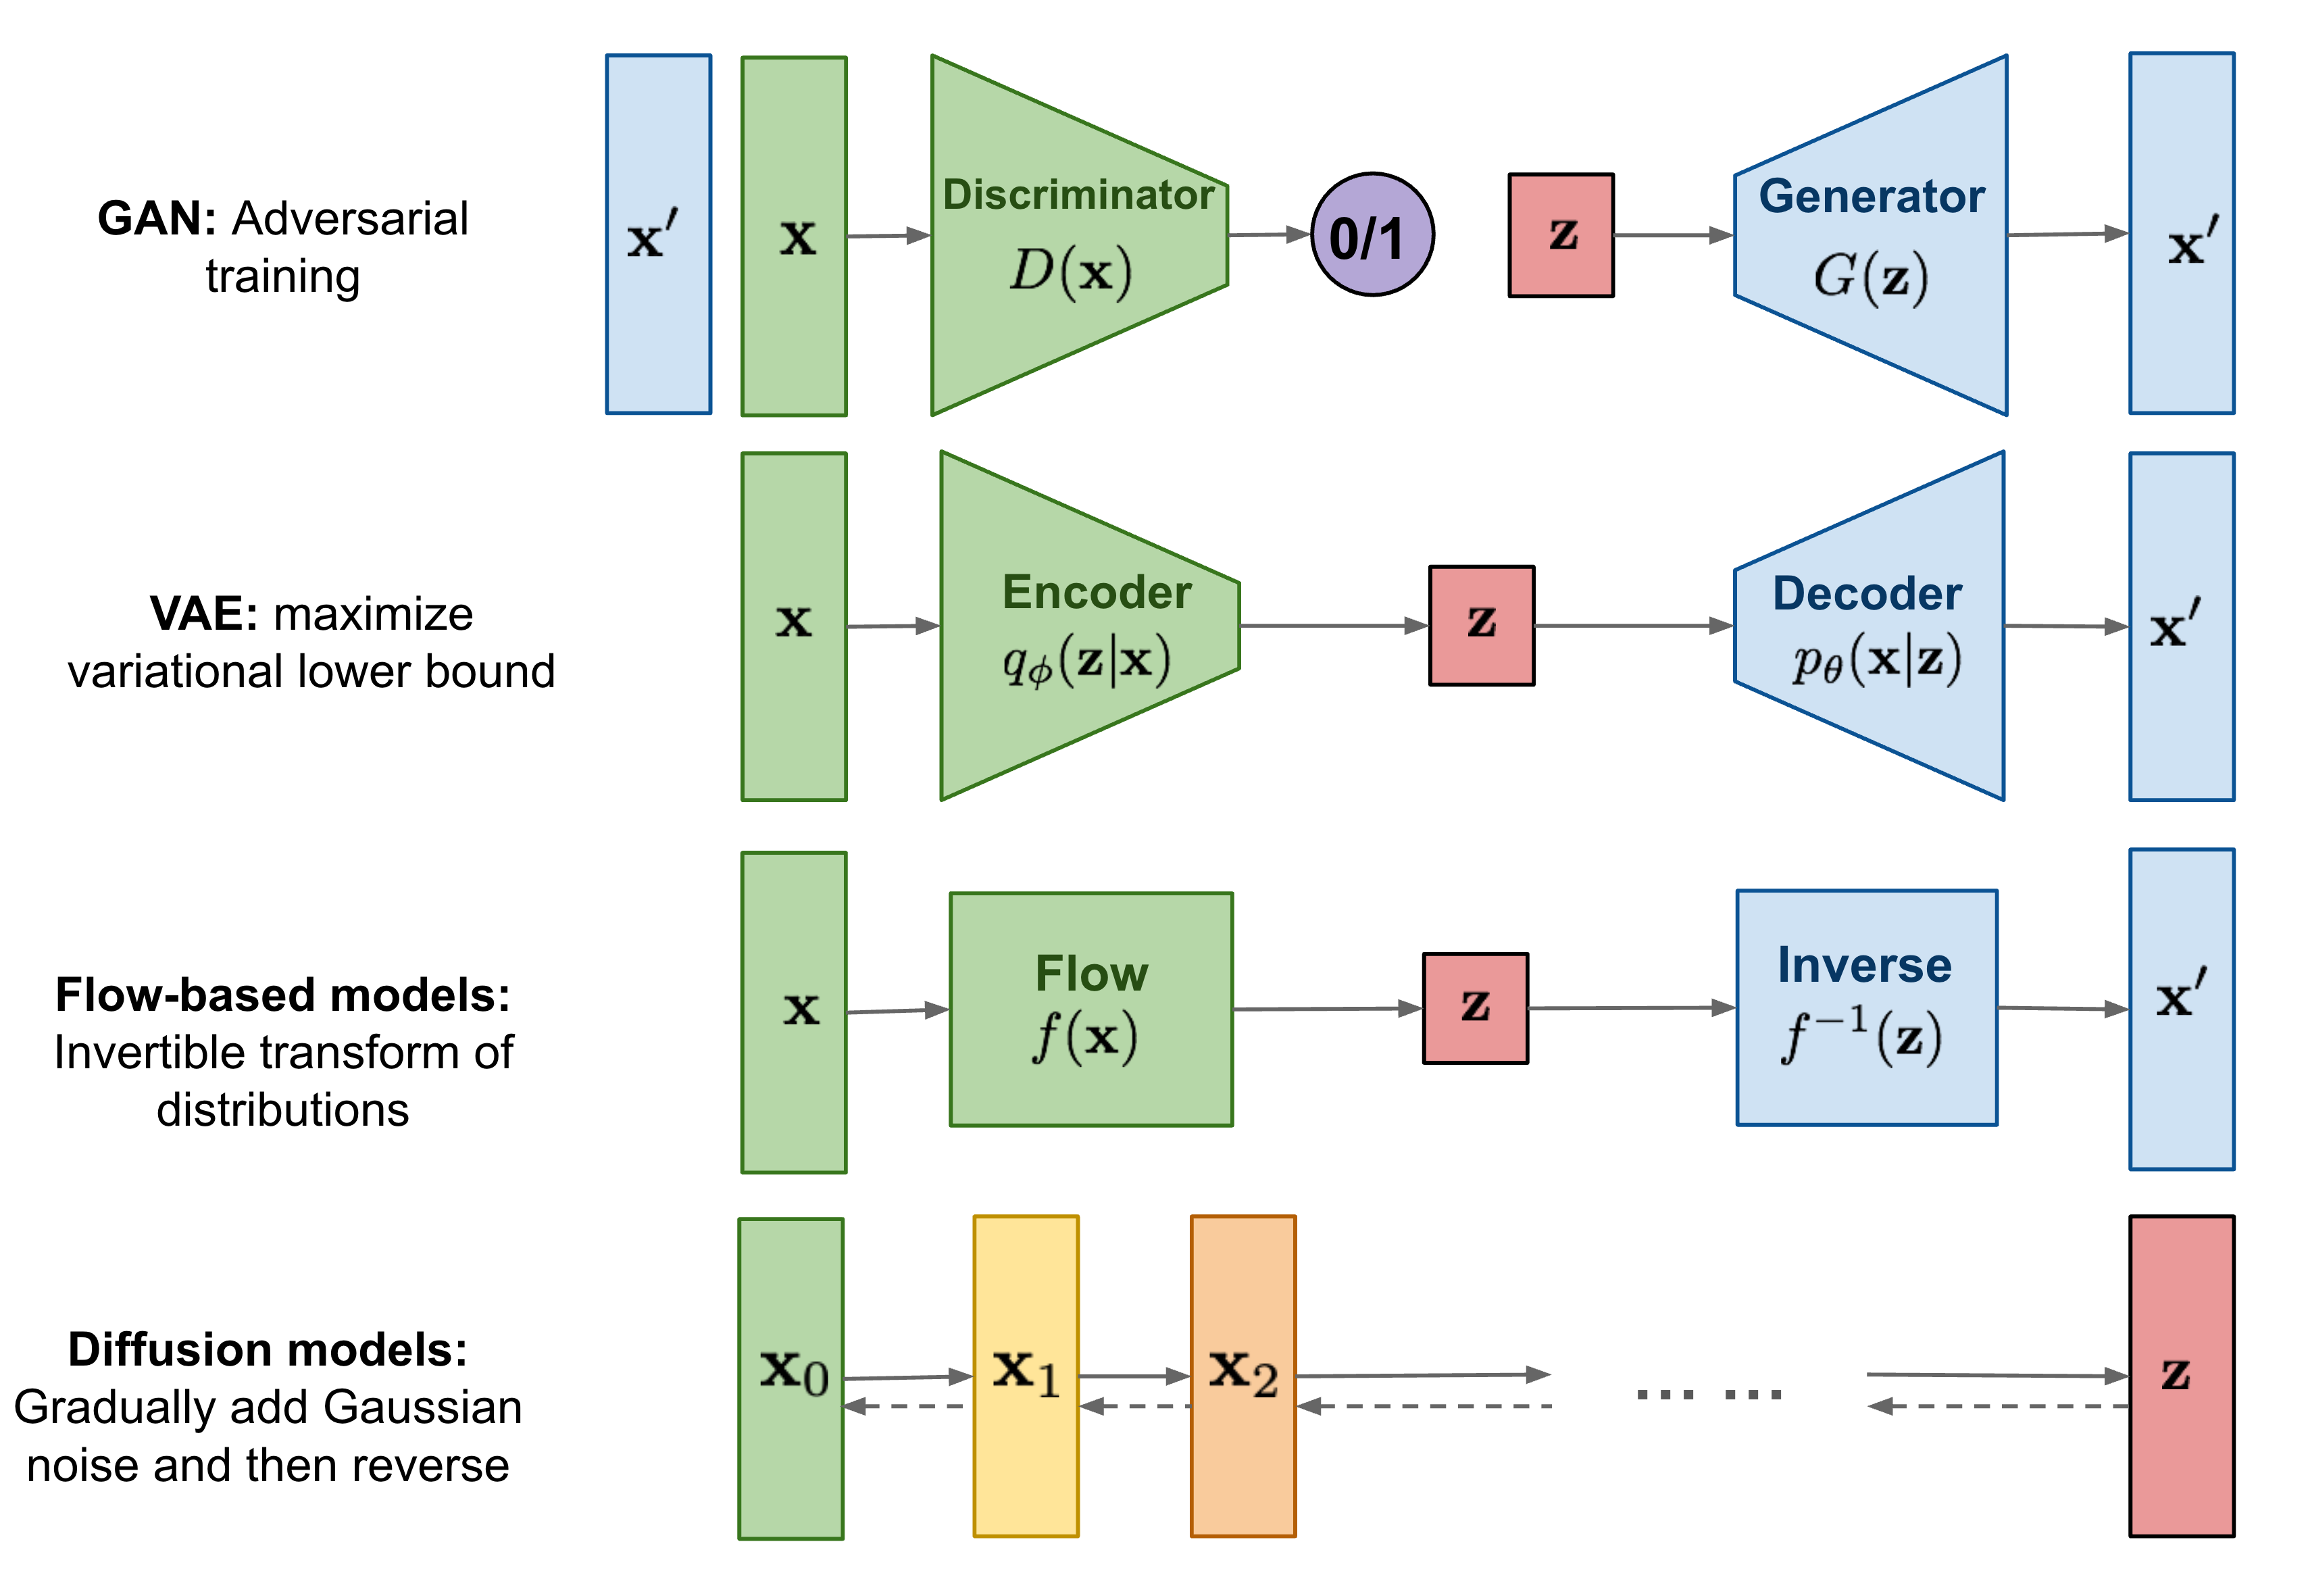
\includegraphics[width=\linewidth]{figs/generative-overview}
	\end{figure}
	\myfootnotewithlink{https://lilianweng.github.io/posts/2021-07-11-diffusion-models/}{Weng L. What are Diffusion Models?, blog post, 2021}
\end{frame}
%=======
\begin{frame}{The worst course overview :)}
	\begin{figure}
		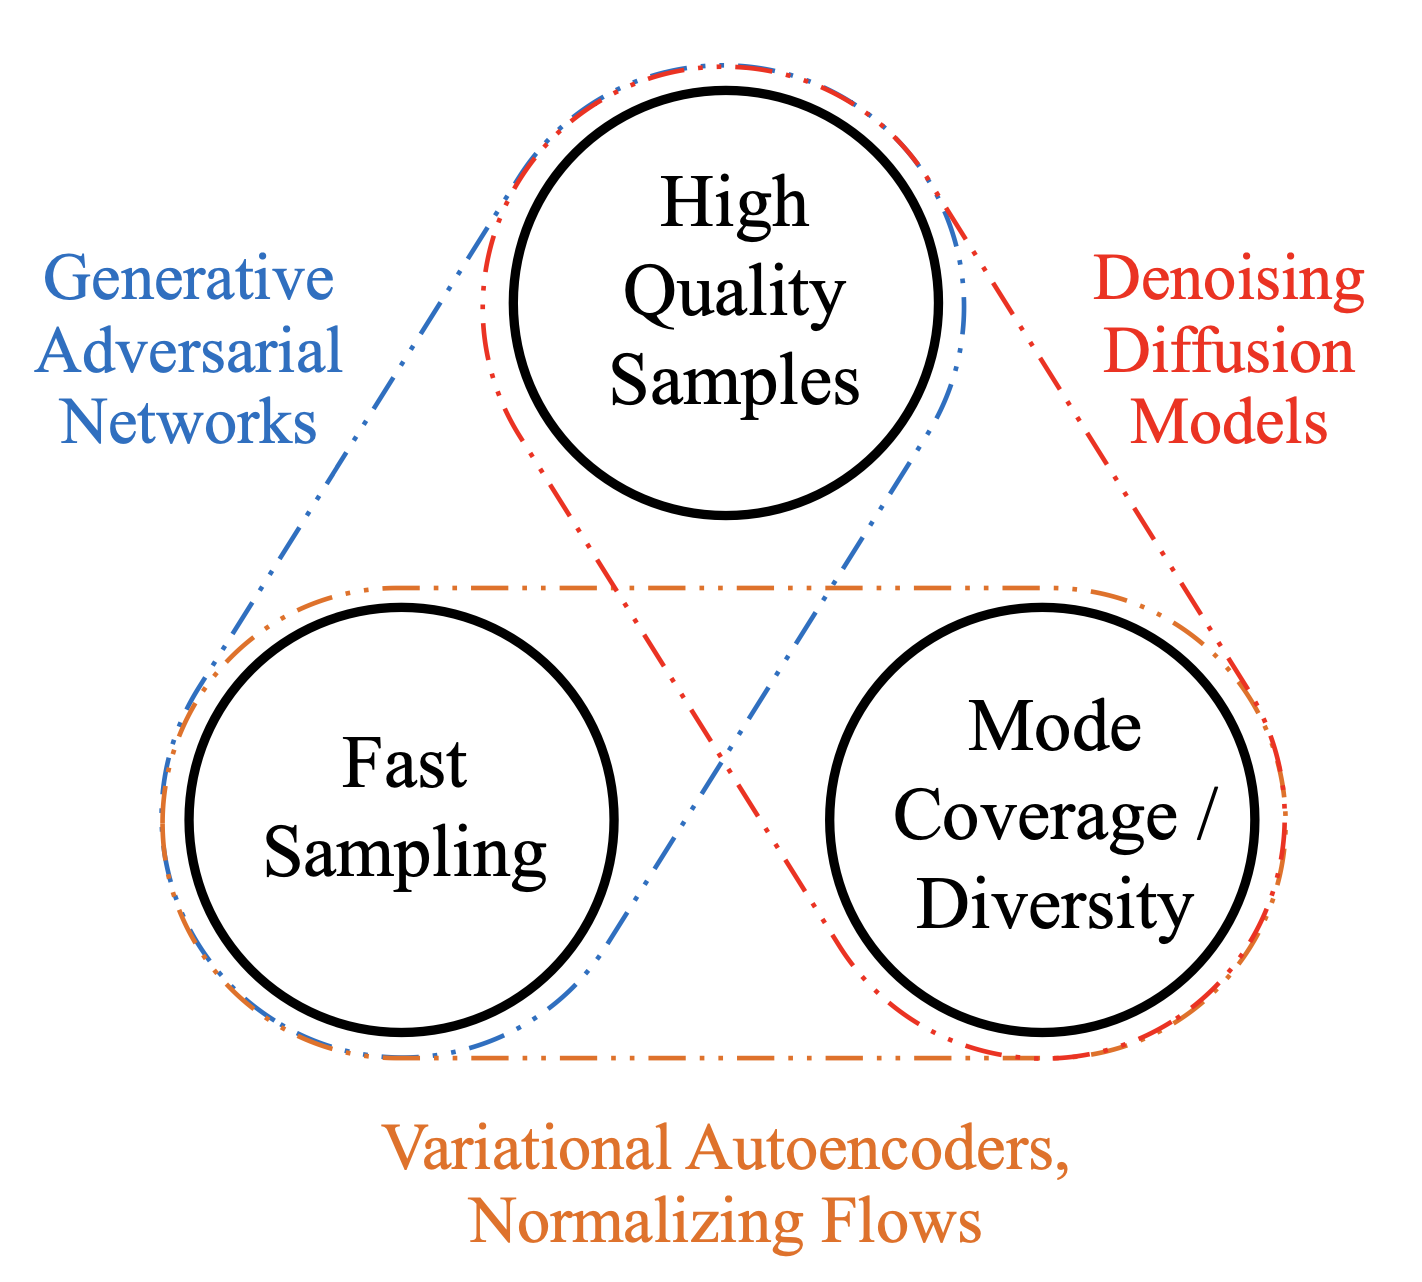
\includegraphics[width=0.7\linewidth]{figs/trilemma}
	\end{figure}
	\myfootnotewithlink{https://arxiv.org/abs/2112.07804}{Xiao Z., Kreis K., Vahdat A. Tackling the generative learning trilemma with denoising diffusion GANs, 2021}
\end{frame}
%=======
\begin{frame}{Summary}
	\begin{itemize}
		\item Langevin dynamics allows to sample from the model using the score function (due to the existence of stationary distribution for SDE).
		\vfill
		\item Score matching proposes to minimize Fisher divergence to get score function.
		\vfill
		\item Sliced score matching and denoising score matching are two techniques to get scalable algorithm for fitting Fisher divergence.
		\vfill
		\item Noise conditioned score network uses multiple noise levels and annealed Langevin dynamics to fit score function.
		\vfill
		\item Objective of DDPM is closely related to the noise conditioned score network and score matching.	
	\end{itemize}
\end{frame}
\end{document} 